\section{Développement du schéma électronique} \label{sec:Dev-Schematique}
Dans cette section, nous décrirons la phase principale du développement ainsi que la démarche suivie pour élaborer le schéma électronique du projet.

\subsection{Blocs développés} \label{ssec:Dev-blocs}
Pour faciliter le développement et la lecture du schéma, il est judicieux de diviser le système en plusieurs blocs. Une structure a ainsi été définie, divisant le circuit en trois blocs principaux : \hyperref[ssec:Dev-MCU]{\textbf{Microcontrôleur \ref{ssec:Dev-MCU}}} (Intelligence du système, connexion du programmeur et LED de vie.), \hyperref[ssec:Dev-Devices]{\textbf{Périphériques \ref{ssec:Dev-Devices}}} (\gls{GNSS}, \gls{imu}, \gls{FTDI}, connecteur USB, Carte SD.) et \hyperref[ssec:Dev-Alim]{\textbf{Alimentations \ref{ssec:Dev-Alim}}} (Connecteur batterie, gestion de charge, régulateurs de tension et système ON/OFF.).

Nous pouvons sur la figure \ref{fig:blocs} observer les différentes interaction entre les blocs, elles sont par la suite décrites dans le tableau \ref{tab:descrConnexion}.

\begin{figure}[h]
	\centering
	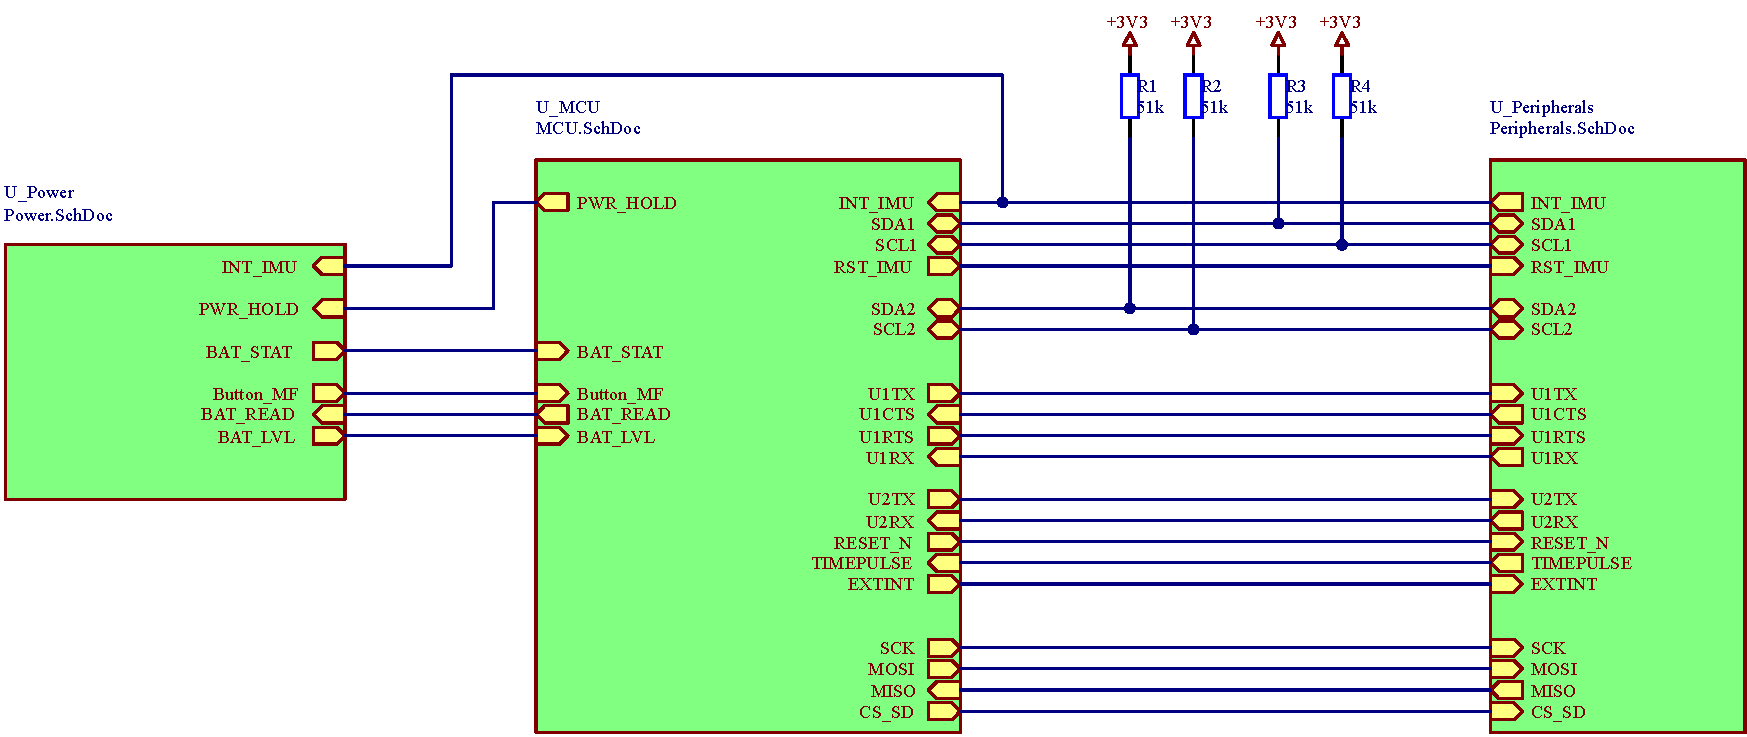
\includegraphics[width=.85\linewidth]{../figures/etude/sch/BLOCS}
	\caption{Blocs du système.}
	\source{Auteur}
	\label{fig:blocs}
\end{figure}

\begin{table}[h]
		\centering
		\resizebox{\columnwidth}{!}{%
			\begin{tabular}{l|l}
				Connexion/s & Description \\
				\hline
				INT\_IMU & Interruption de la centrale inertielle, informe le \gls{mcu} et peut allumer le système. \\ 
				RST\_IMU & Permet de réinitialiser la \gls{imu}. \\
				PWR\_HOLD & Le \gls{mcu} peut se maintenir alimenté par cette connexion. \\
				BAT\_STAT & Fournit le statut de la batterie au \gls{mcu}. \\
				Button\_MF & Fournit le niveau logique du bouton au \gls{mcu}. \\
				BAT\_READ & Le \gls{mcu} peut activer la lecture de la tension de la batterie. \\
				BAT\_LVL & Lecture analogique de la tension de batterie. \\
				SDA1, SCL1 & Communication I2C avec l'\gls{imu}. \\
				SDA2, SCL2 & Communication I2C optionnelle avec le \gls{GNSS}. \\
				U1TX/RX... & Communication UART avec le \gls{FTDI} pour l'USB. \\
				U2TX/RX & Communication UART avec le \gls{GNSS}. \\
				RESET\_N & Permet de réinitialiser le \gls{GNSS}. \\
				TIMEPULSE & Permet de mesurer le temps par un signal pulsé. \\
				EXTINT & Permet de gérer le mode d'alimentation du \gls{GNSS} \\
				SCK, MOSI... & Communication SPI avec la carte SD. \\ 
				R1,2,3,4 & Résistances de PULL-UP pour communication I2C. \\
			\end{tabular}
		}
		\caption{Description des connexions}
		\label{tab:descrConnexion}
	\end{table}

\clearpage

\subsection{Microcontrôleur} \label{ssec:Dev-MCU}

\subsubsection{Connexion} 
Pour utiliser le microcontrôleur, il est nécessaire de définir ses entrées/sorties en se référant à son \gls{datasheet}. Ce dernier permet de connaître les connexions dédiées à certains bus de communication ou à des entrées analogiques. 

\begin{figure}[h]
	\centering
	\begin{subfigure}[b]{0.6\textwidth}
		\centering
		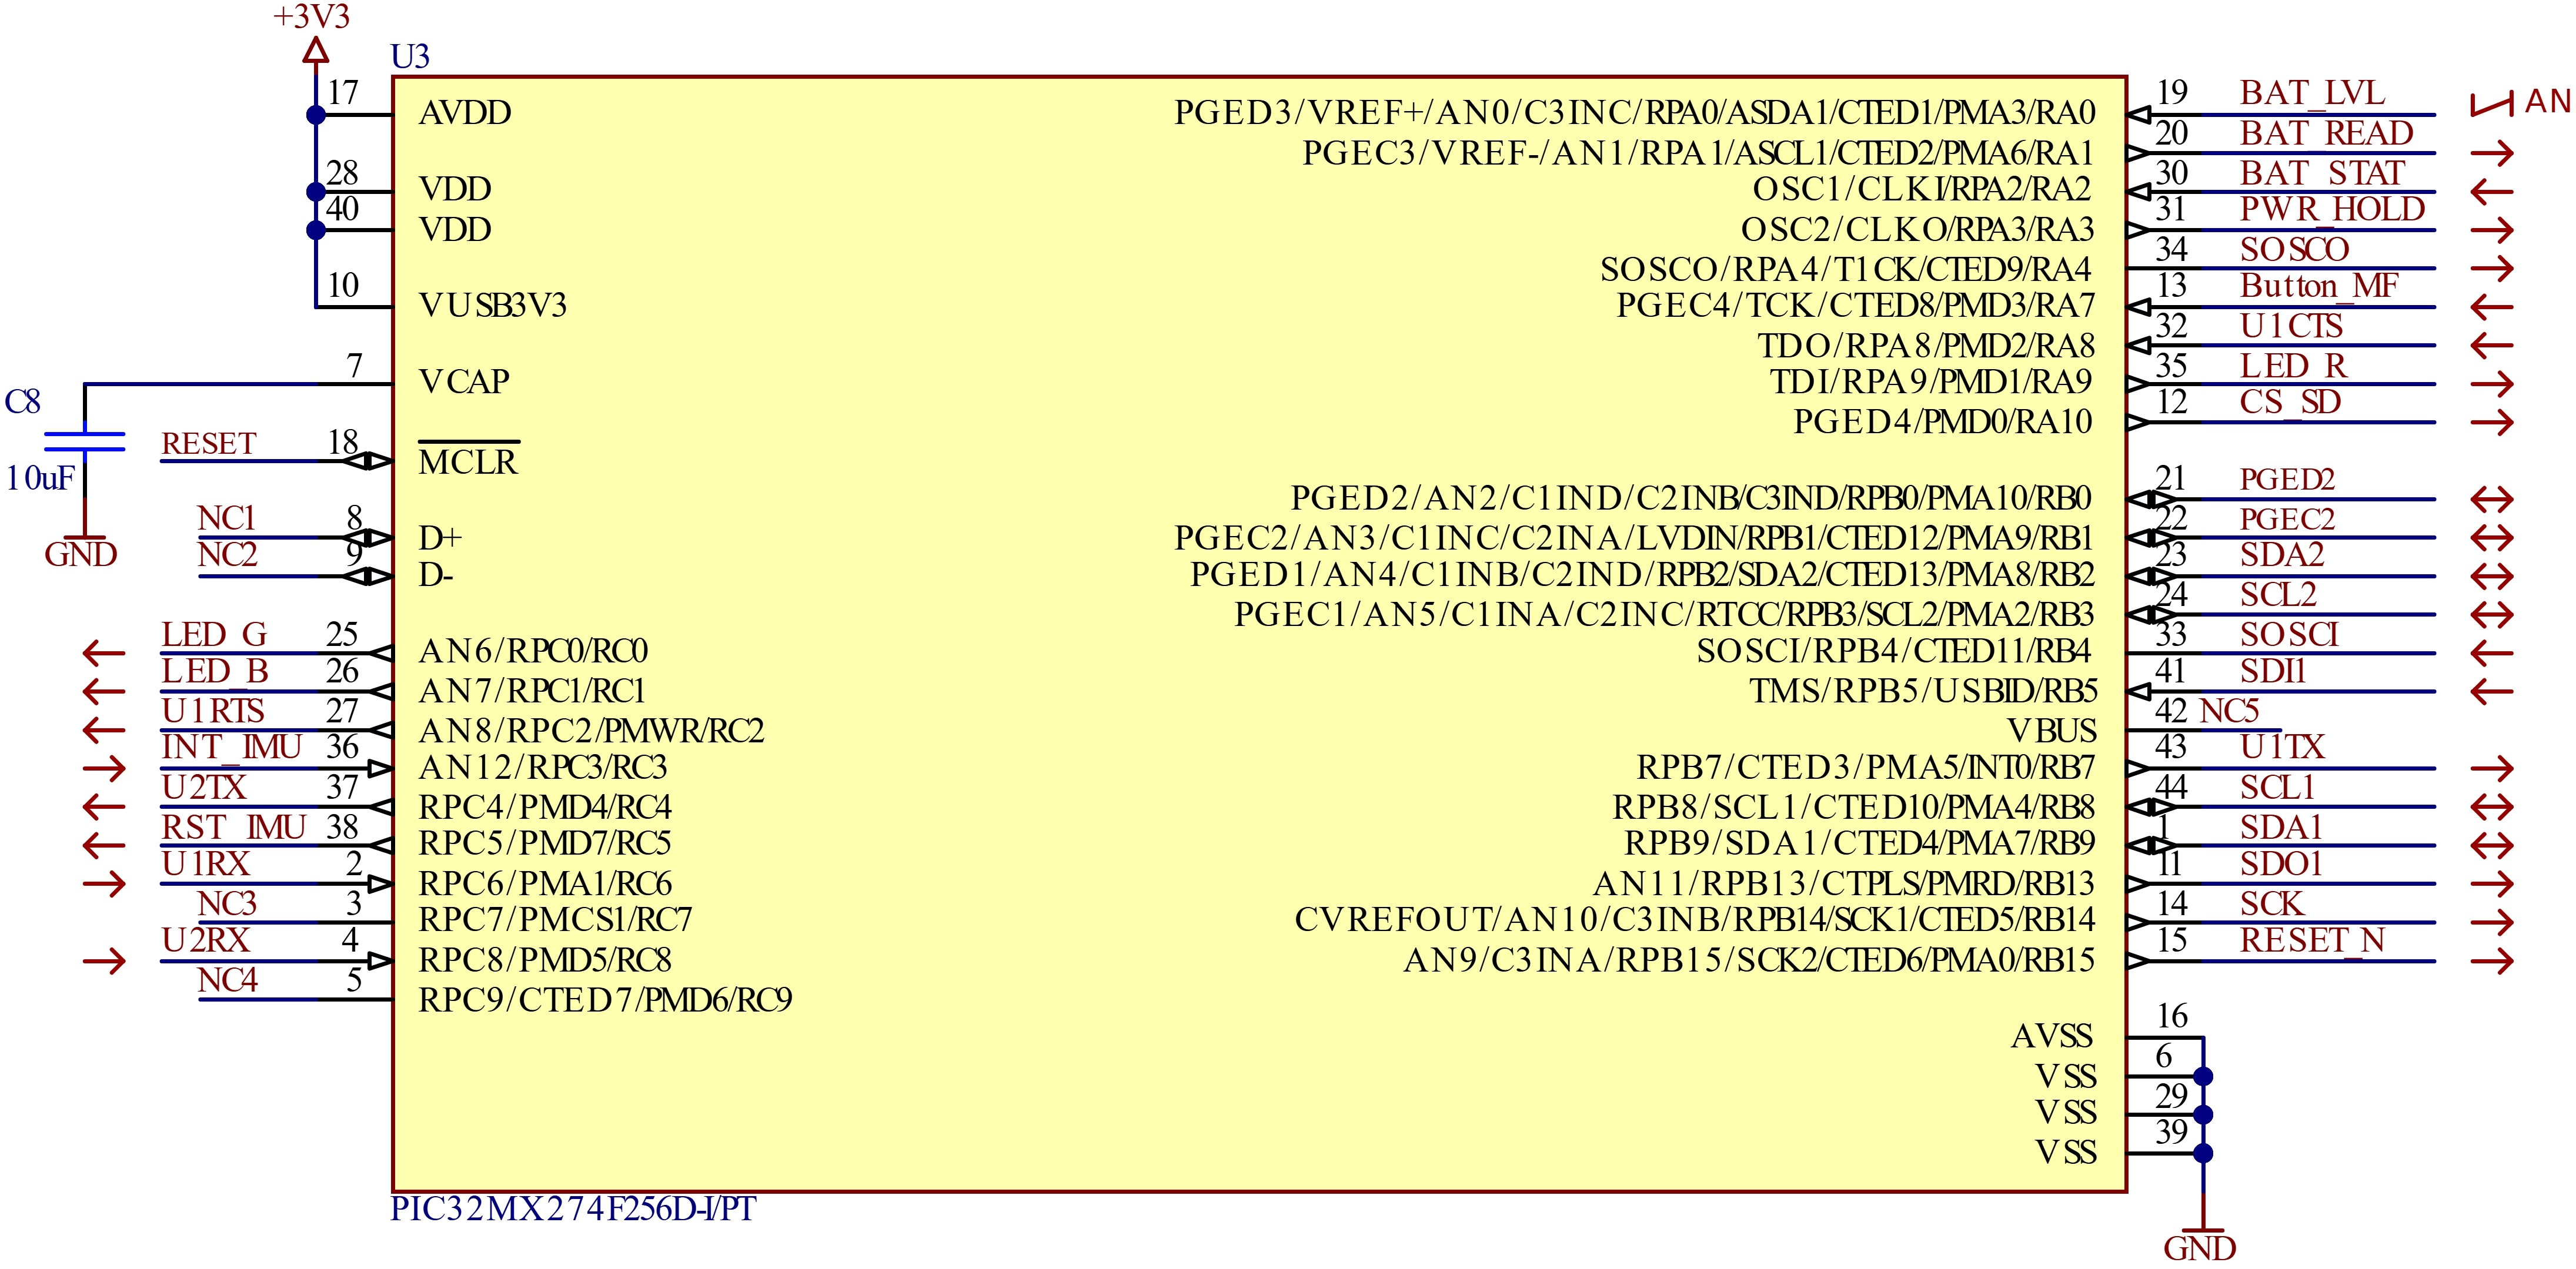
\includegraphics[width=1\linewidth]{../figures/etude/sch/MCU}
		\caption{Connexions du microcontrôleur}
		\label{fig:mcu}
	\end{subfigure}
	\hfill
	\begin{subfigure}[b]{0.3\textwidth}
		\centering
		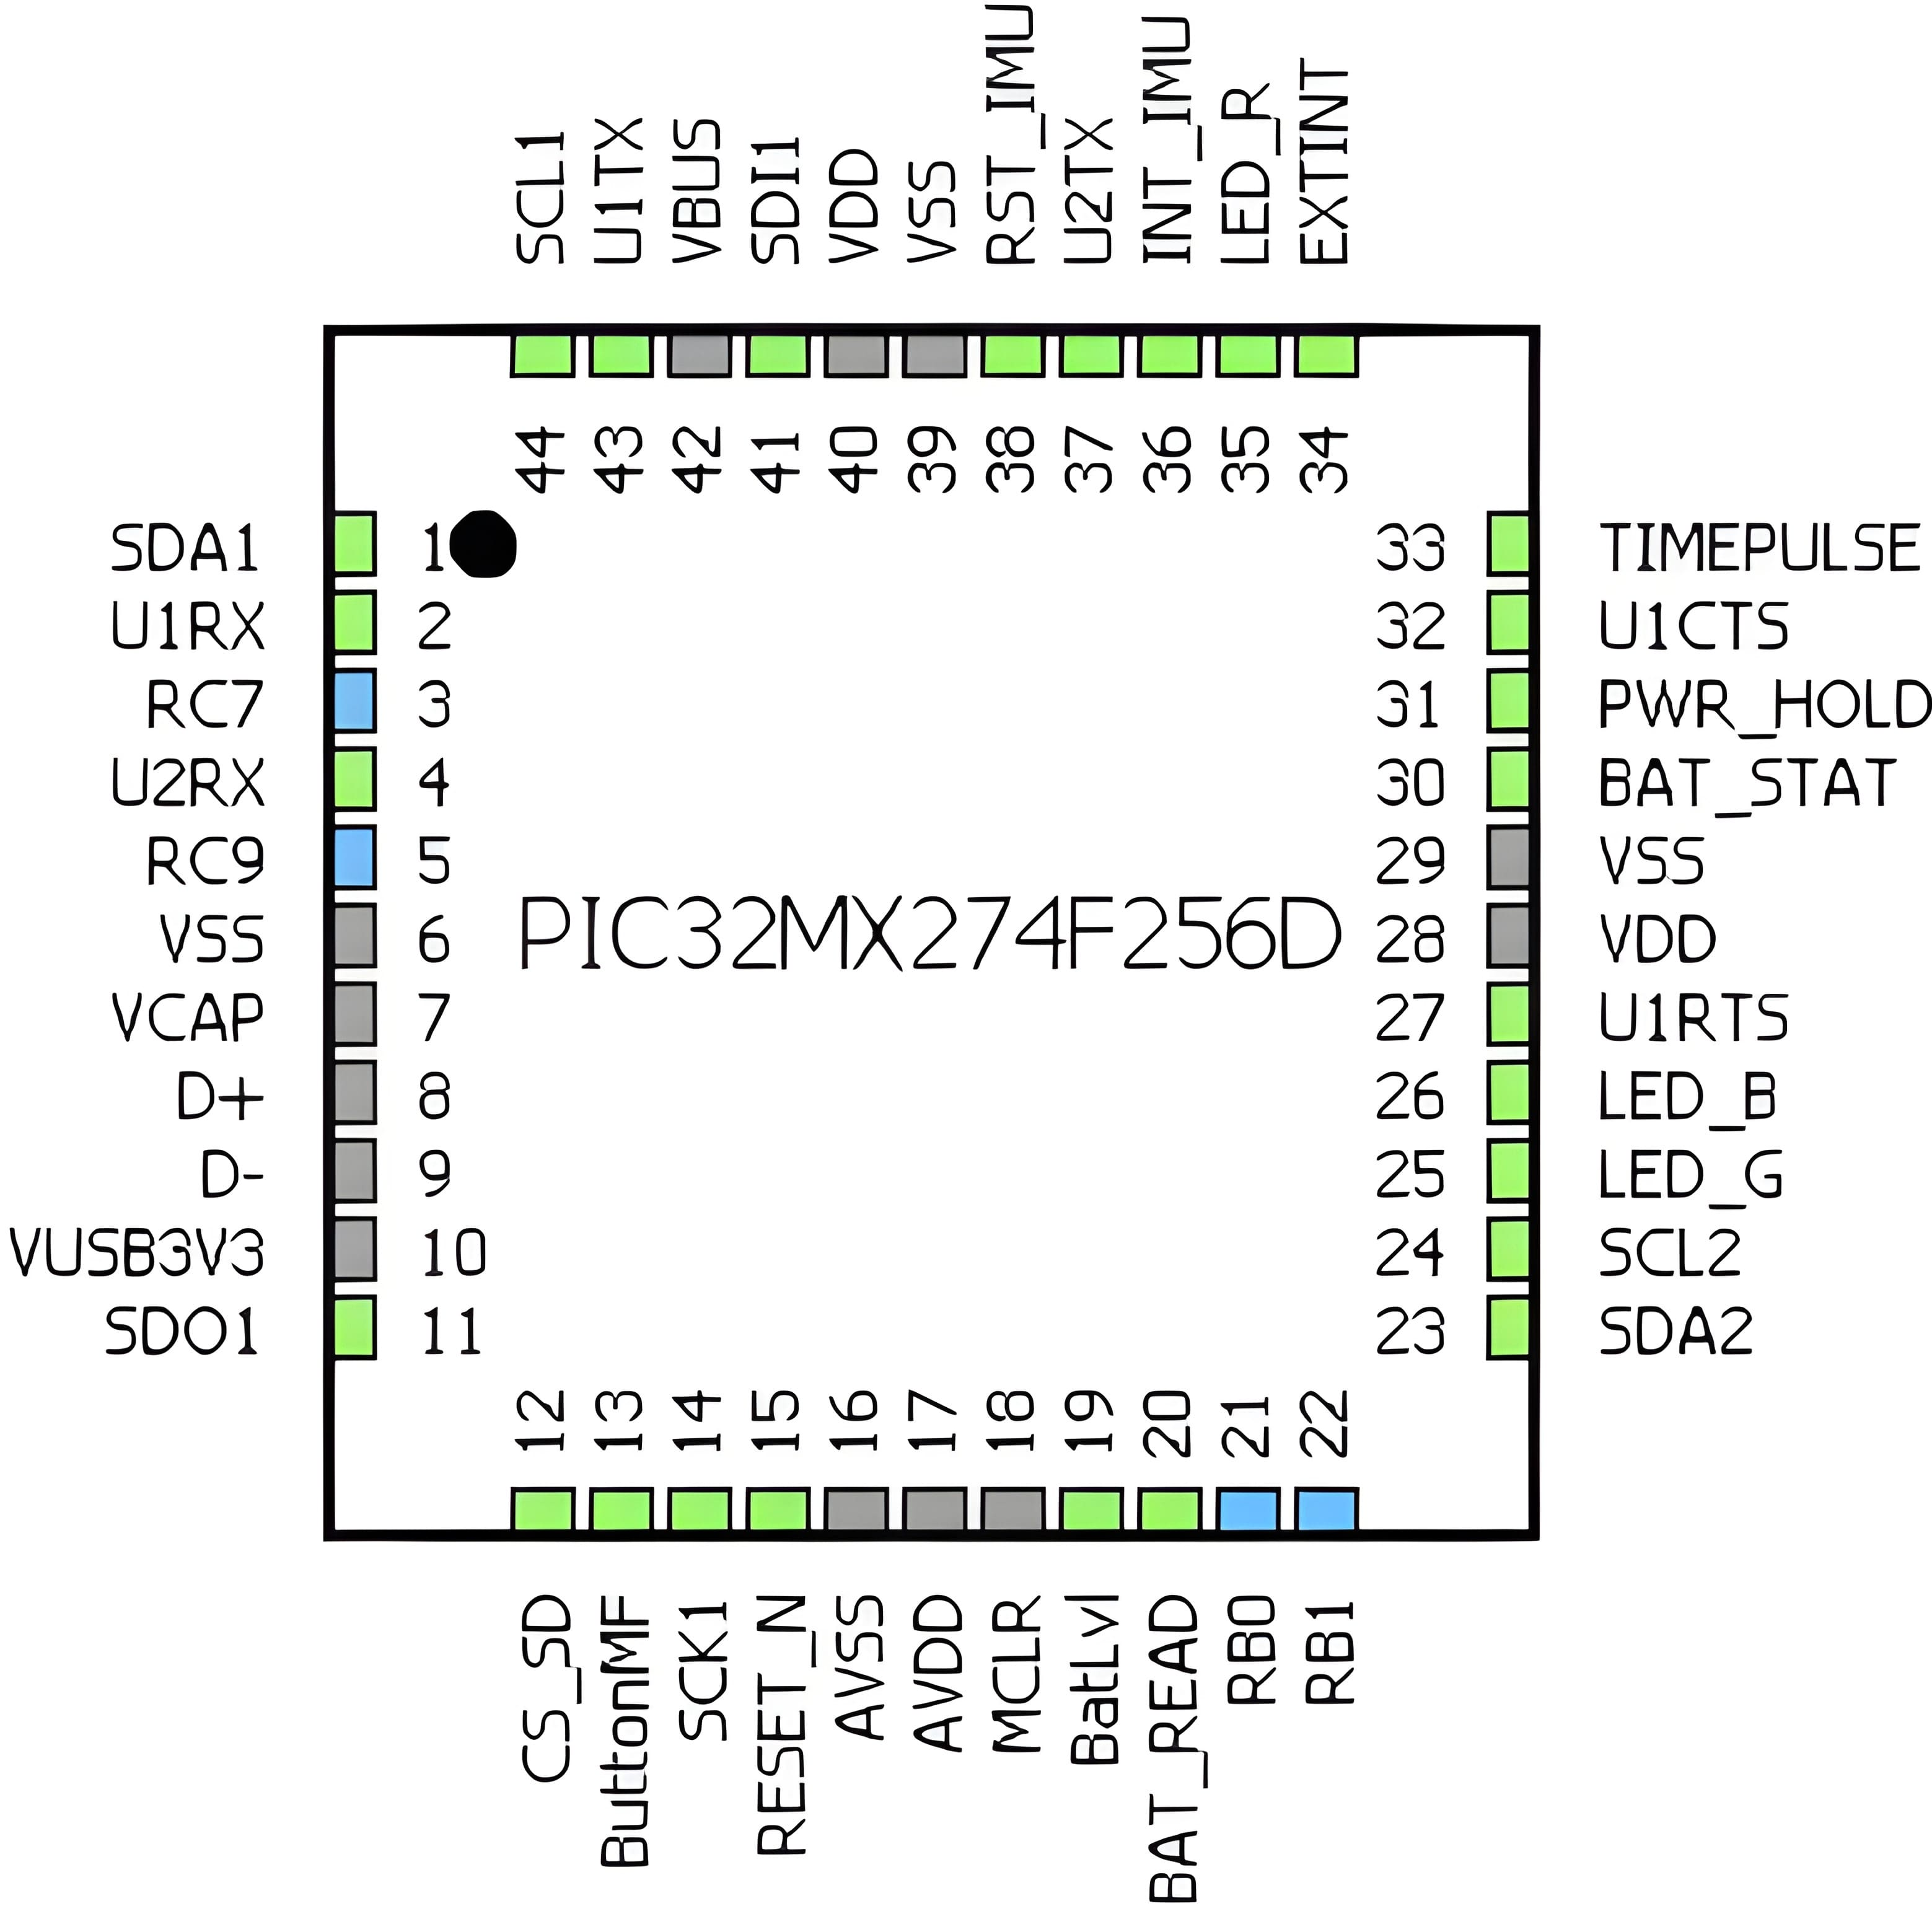
\includegraphics[width=1\linewidth]{../figures/etude/sch/MCU-HARMONY}
		\caption{Config. \gls{harmony}.}
		\label{fig:mcu-harmony}
	\end{subfigure}
	\hfill
	\caption{Configuration des PINs du microcontrôleur.}
	\source{Auteur}
	\label{fig:sch-connMcu}
\end{figure}

Pour valider les connexions de la figure \ref{fig:mcu}, une vérification a été réalisée à l'aide du configurateur graphique \gls{harmony}, comme le montre la figure \ref{fig:mcu-harmony}. Cette étape a confirmé la possibilité d'attribuer certaines fonctions à des PINs spécifiques. Les PINs non utilisées du microcontrôleur sont redirigées vers un connecteur. Dans le contexte du prototype, cela permet de les exploiter ailleurs sur la carte.


\subsubsection{Programmateur et reset} 

\begin{figure}[h]
	\centering
	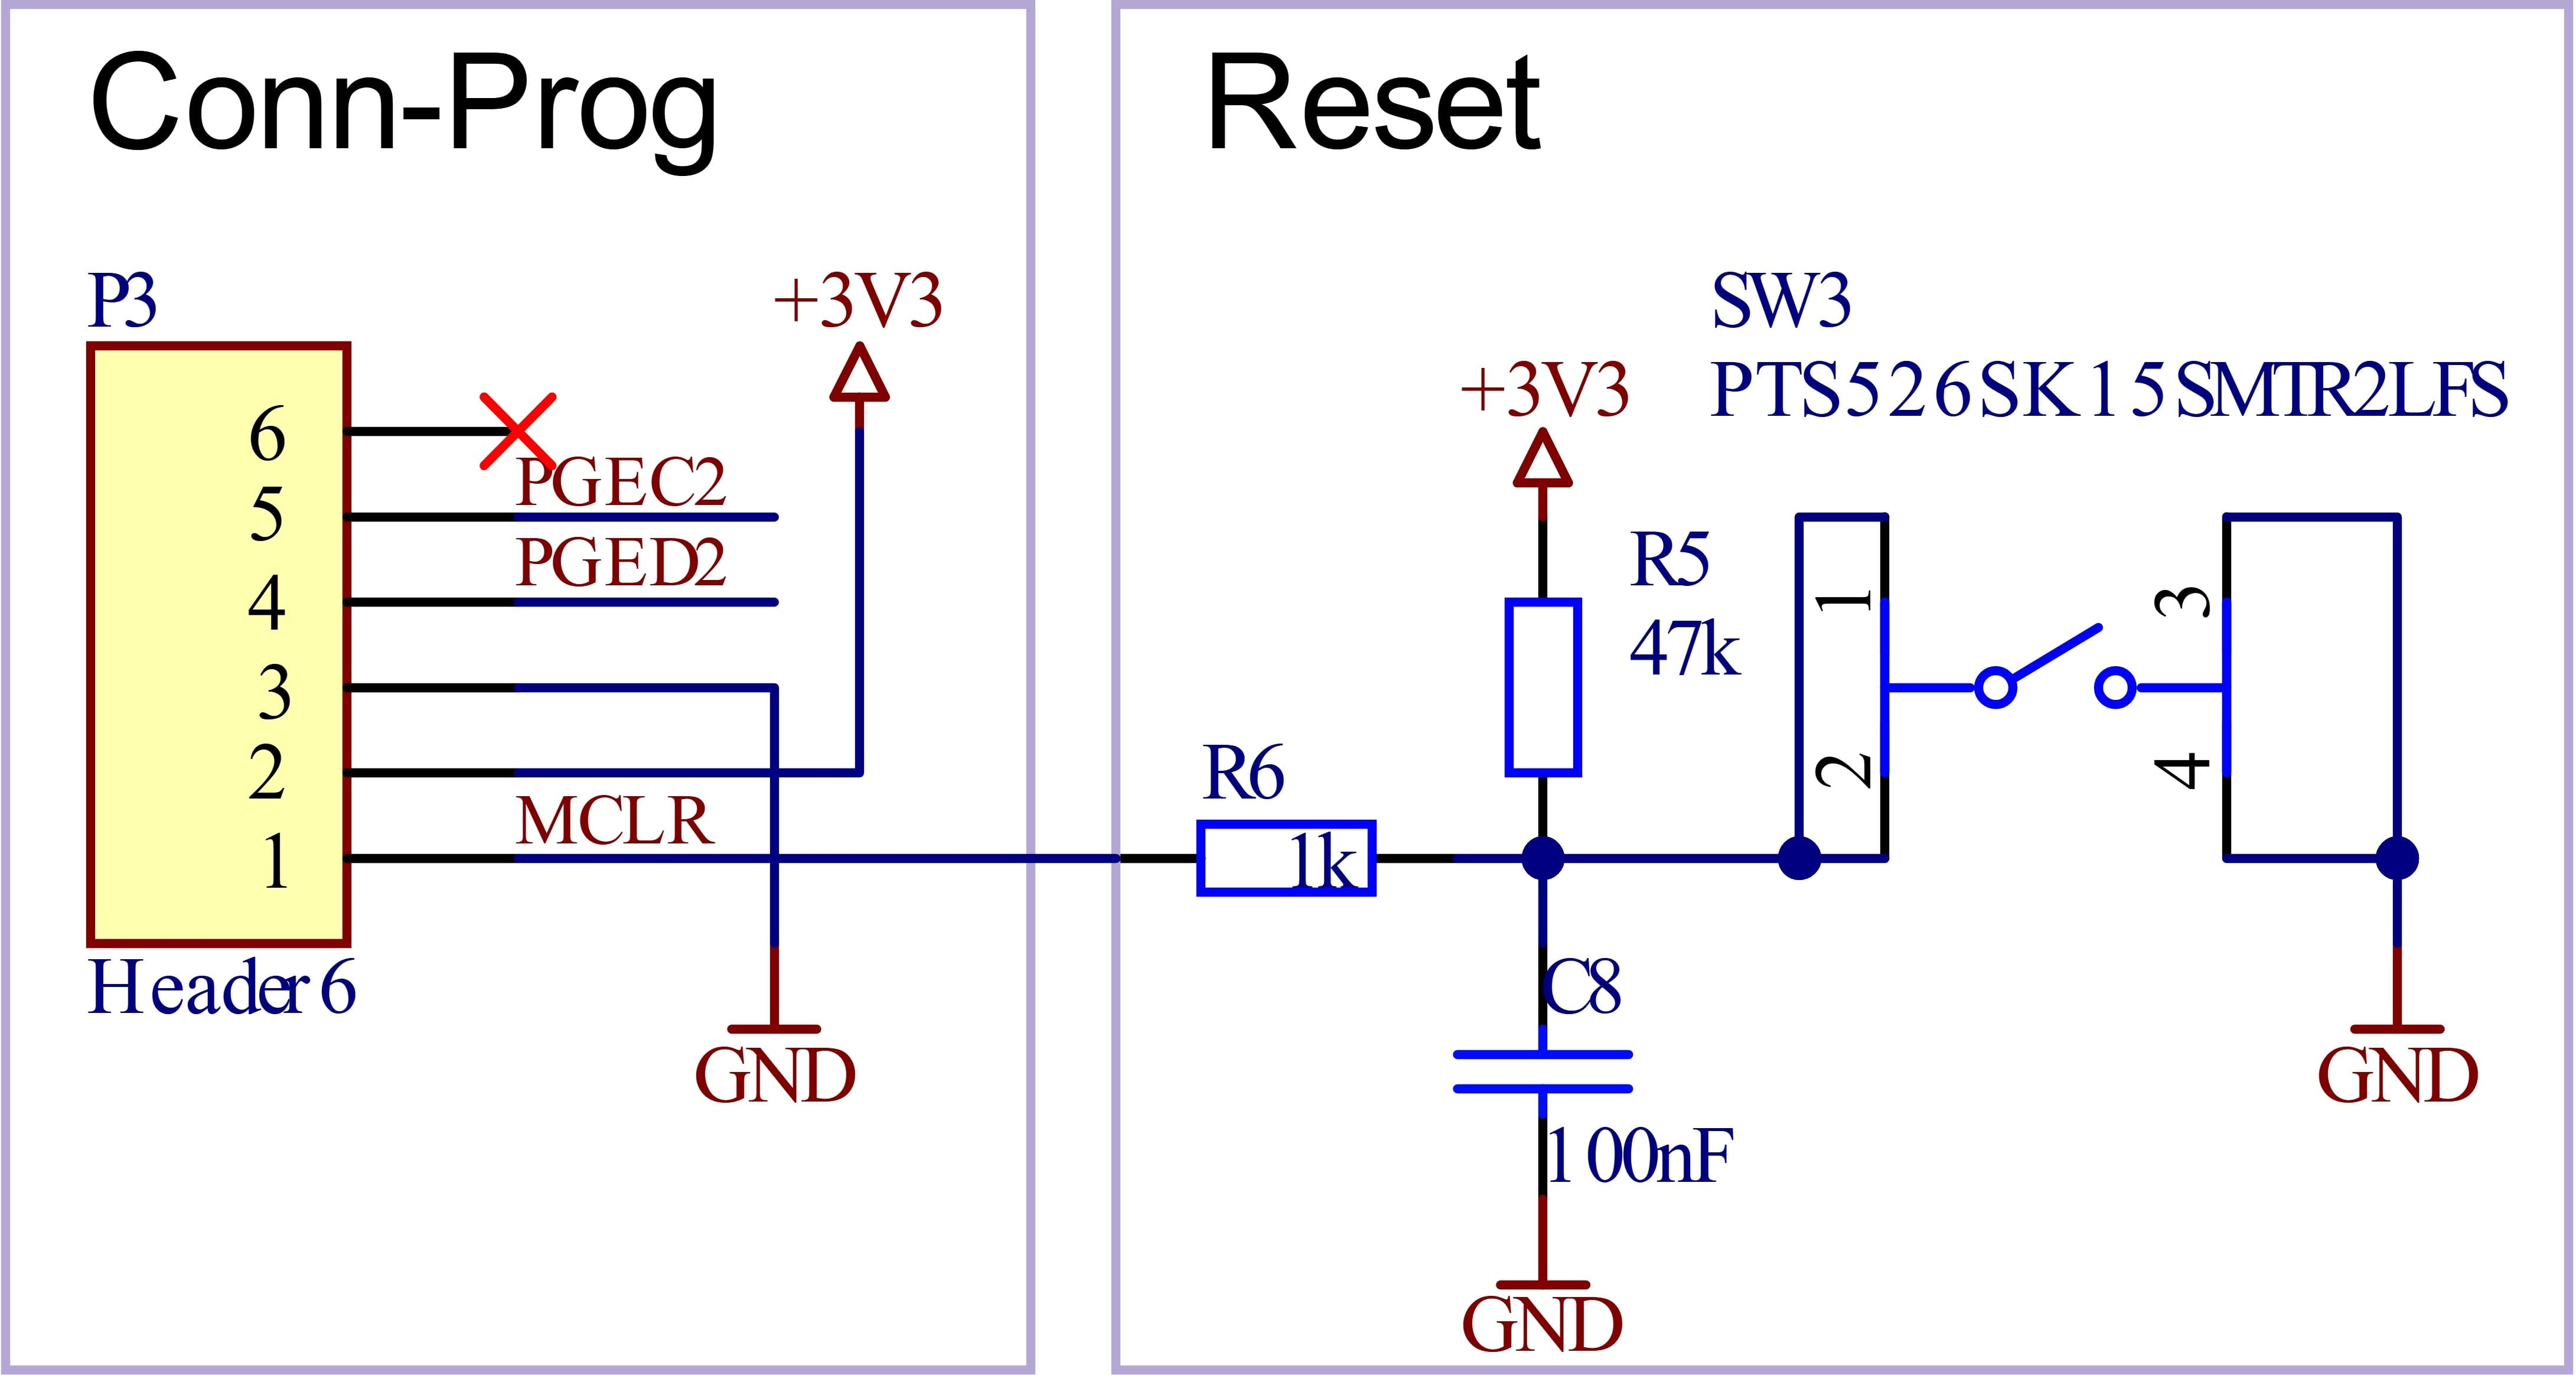
\includegraphics[width=.65\linewidth]{../figures/etude/sch/Prog-Reset}
	\caption{Schéma programmateur et reset.}
	\source{Auteur}
	\label{fig:prog-reset}
\end{figure}

Sur la figure \ref{fig:prog-reset}, nous pouvons observer le connecteur de programmation \textit{P3}. La connexion \textbf{MCLR} (Master Clear), qui permet de réinitialiser le \gls{mcu} lors de sa programmation, est suivie d'un bouton pour permettre une réinitialisation manuelle.

\clearpage

\subsubsection{LED de vie} 

\begin{figure}[h]
	\centering
	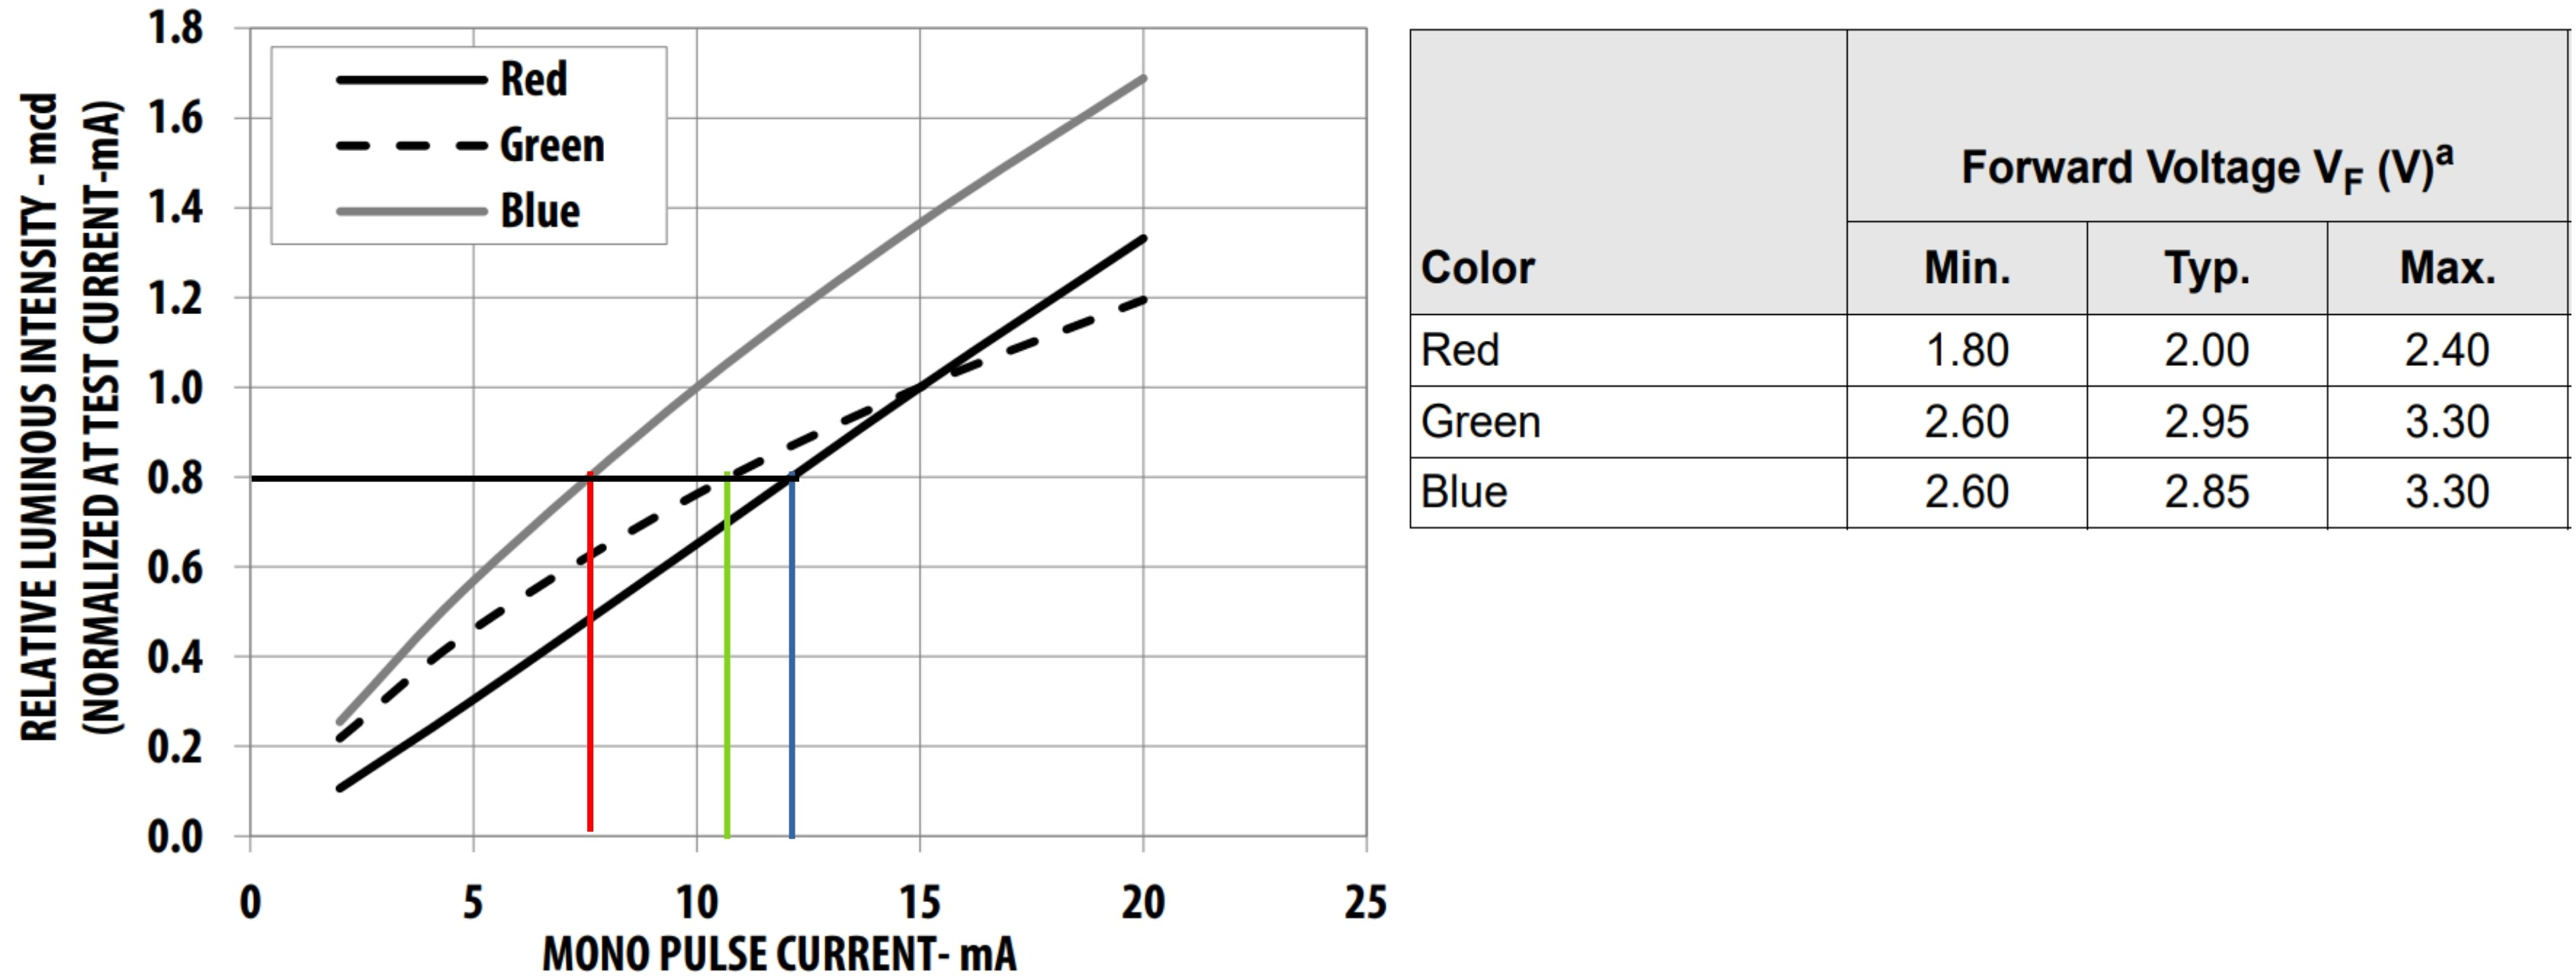
\includegraphics[width=.9\linewidth]{../figures/etude/DIM-LED}
	\caption{Données de la LED}
	\source{\gls{datasheet} \href{https://docs.broadcom.com/doc/ASMB-KTF0-0A306-DS100}{ASMB-KTF0-0A306}}
	\label{fig:dim-led}
\end{figure}

\begin{figure}[h]
	\centering
	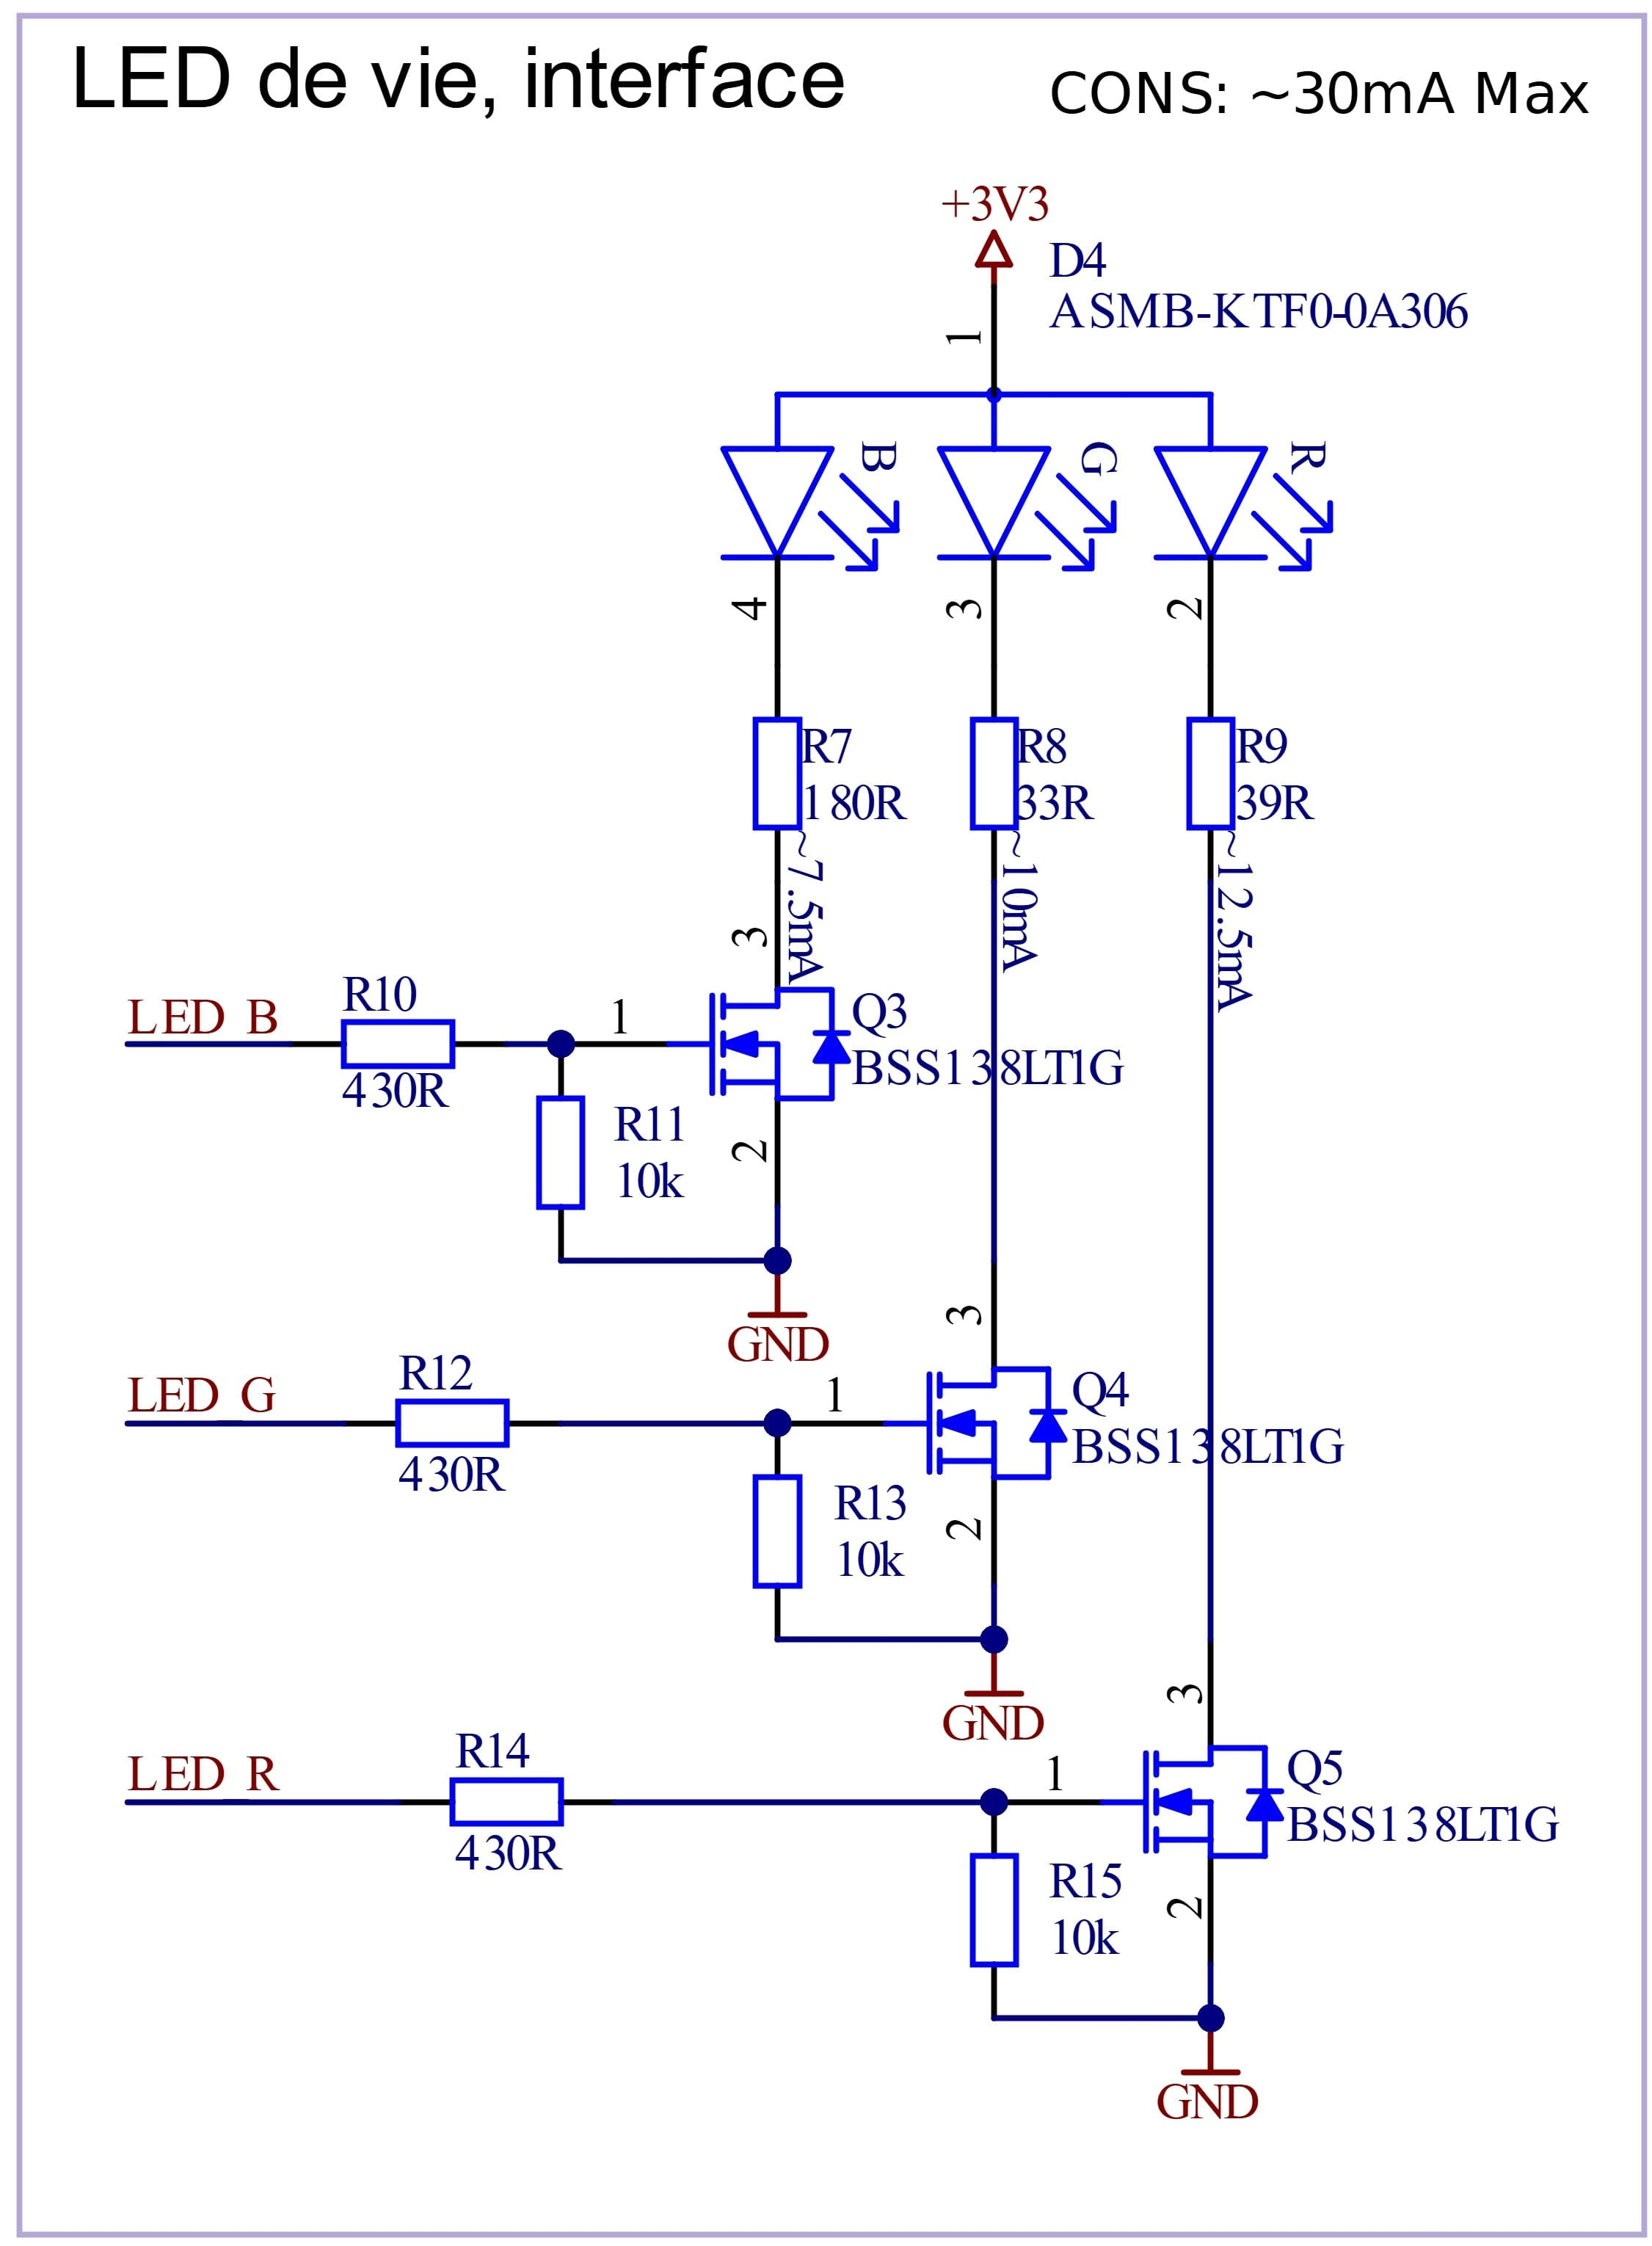
\includegraphics[width=0.4\linewidth]{../figures/etude/sch/LED-Vie}
	\caption{Schéma de la LED de vie.}
	\source{Auteur}
	\label{fig:led-vie}
\end{figure}

Les résistances de la figure \ref{fig:led-vie} ont été dimensionnées en respectant les caractéristiques des LEDs pour chacune des couleurs (voir figure \ref{fig:dim-led}). Ces dernières éclairent à 80\% de leur luminosité nominale dans un souci d'économie d'énergie, leur utilité étant réduite à ce stade de prototypage.

\begin{center}
	\underline{Exemple dimensionnement résistance LED bleue}
	\begin{equation*}
		R_{blue} = \frac{(Vcc - V_{blue})}{I_b} = \frac{(3.3 - 2.85)}{12*10^-3} = 37.5 \Omega
	\end{equation*}
\end{center}

\clearpage

\subsection{Périphériques} \label{ssec:Dev-Devices}
Dans cette section, nous allons décrire les schématiques des périphériques du système.
 
\subsubsection{Carte SD}

\begin{figure}[h]
	\centering
	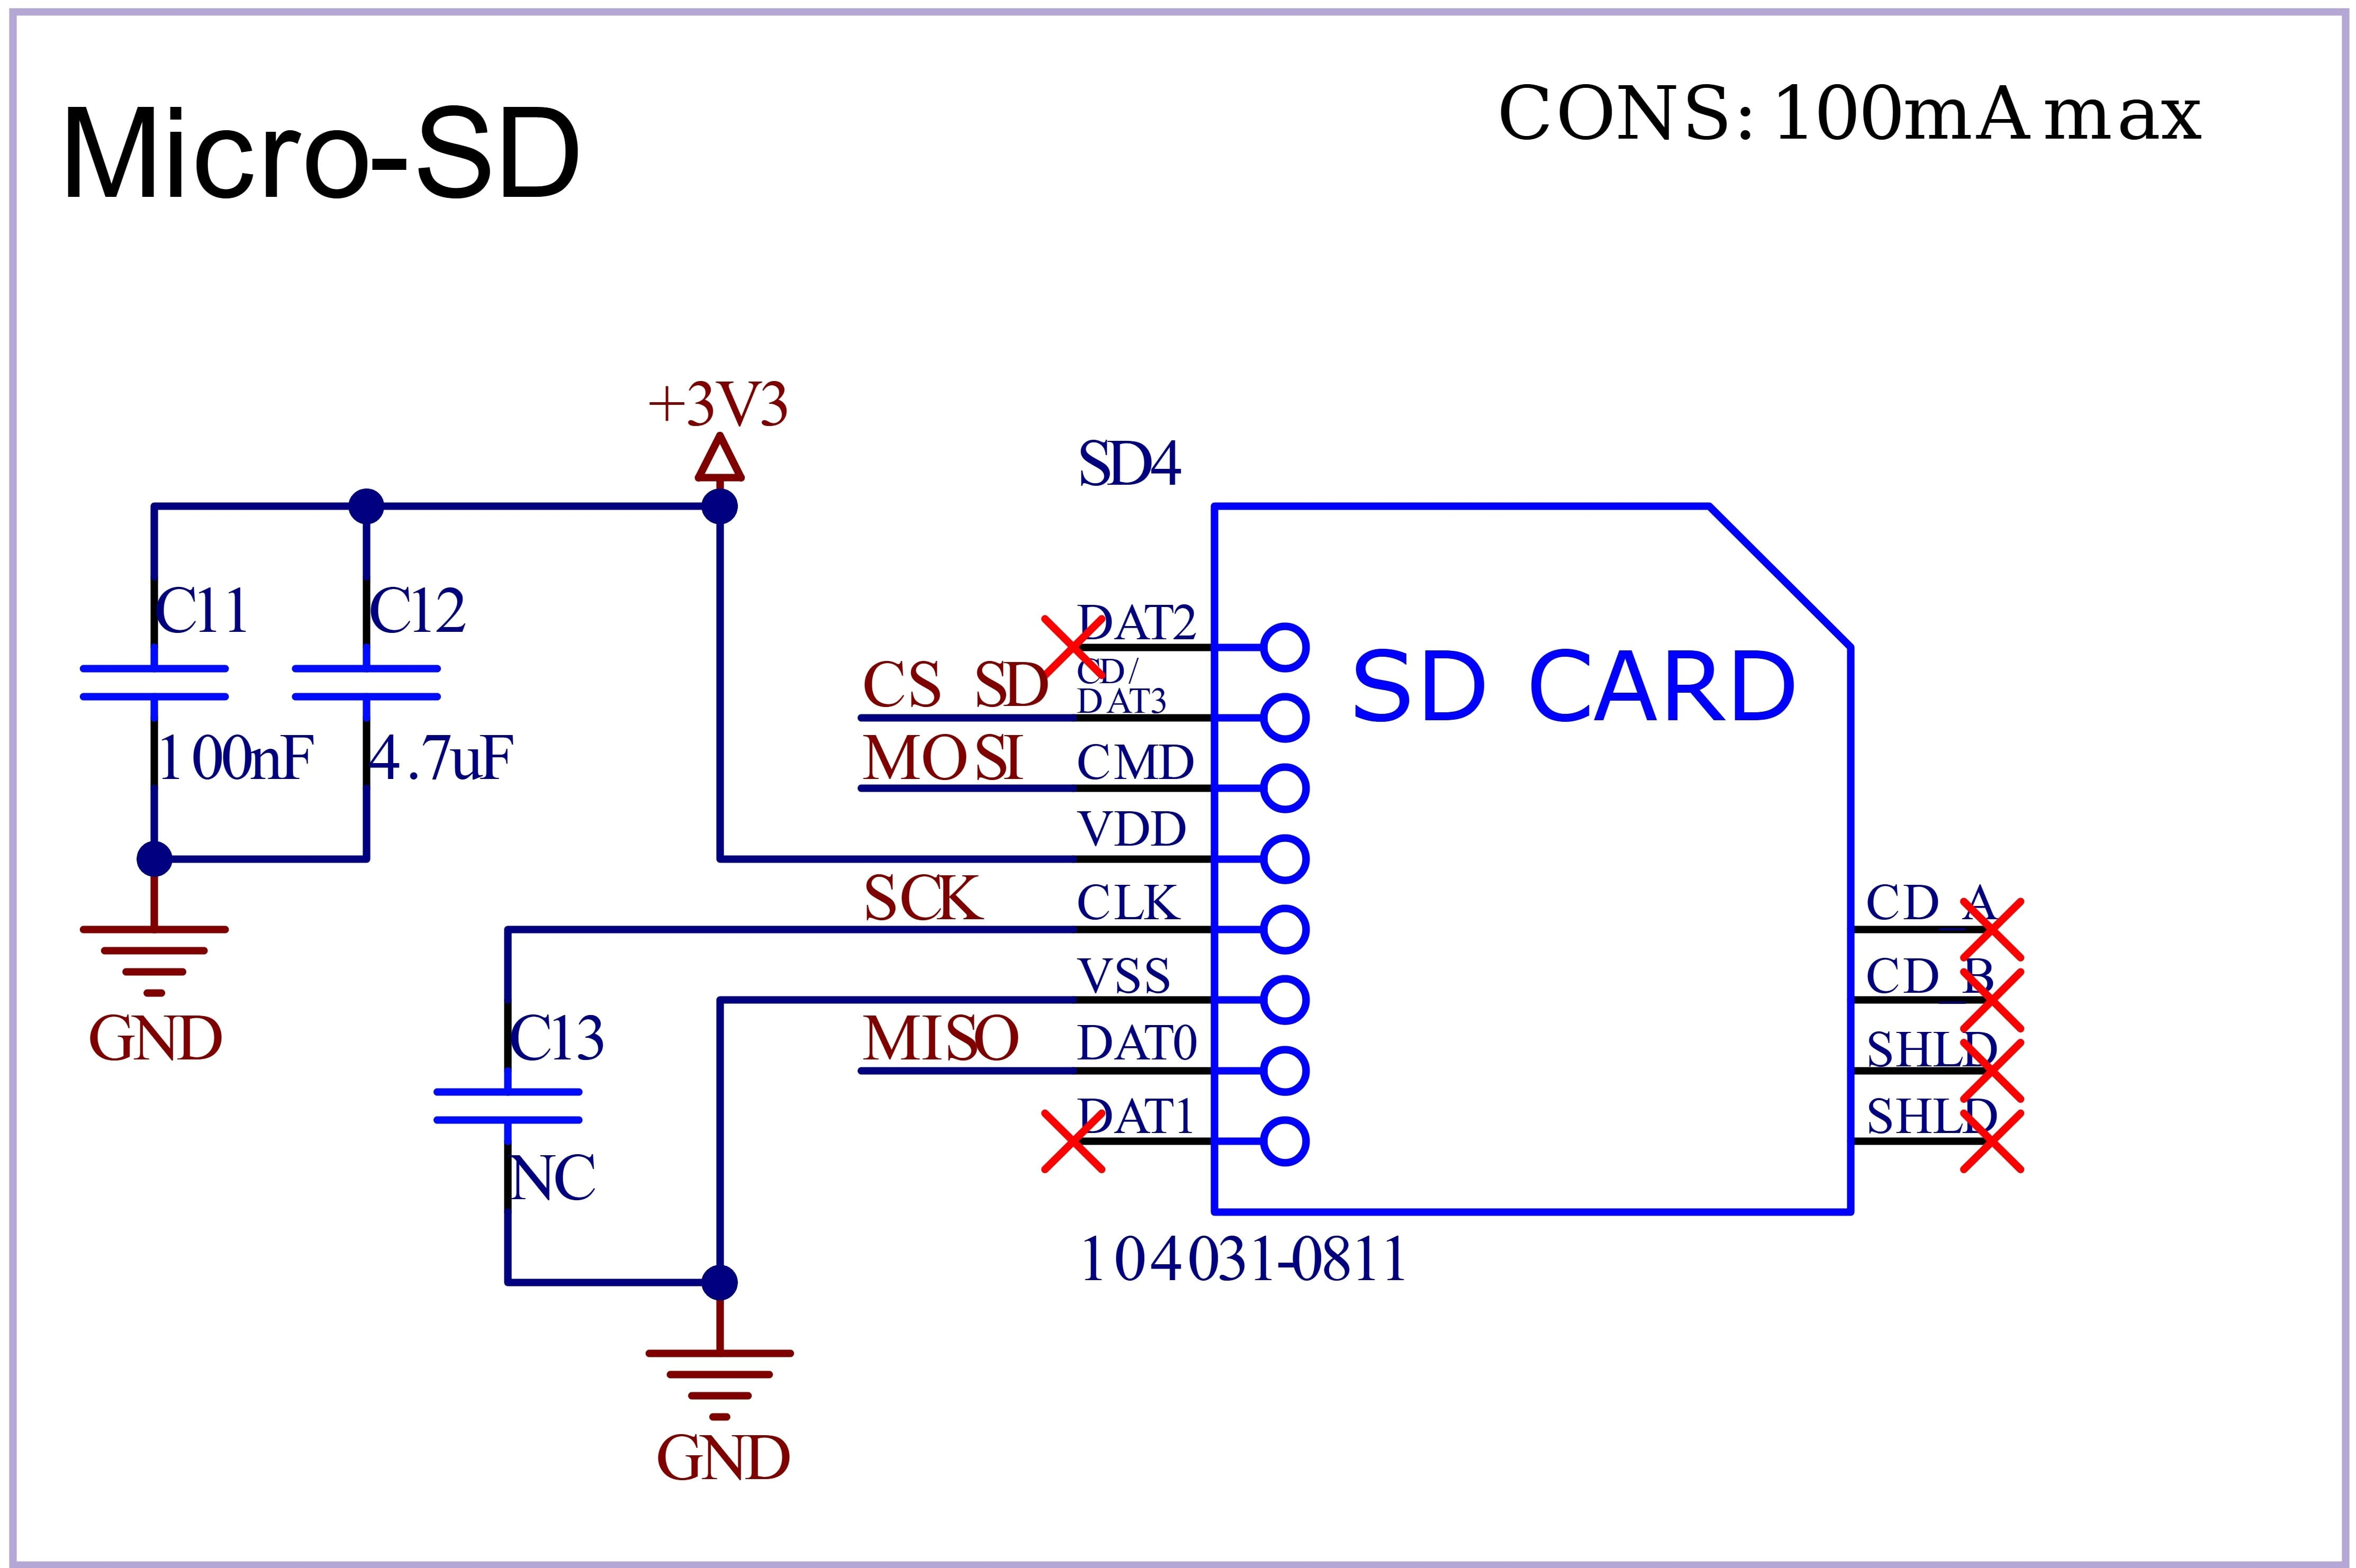
\includegraphics[width=0.5\linewidth]{../figures/etude/sch/Carte-SD}
	\caption{Branchement carte SD.}
	\source{Auteur}
	\label{fig:carte-sd}
\end{figure}

La carte SD de la figure \ref{fig:carte-sd} est branchée en respectant la connectique pour une communication SPI simple. De plus, un condensateur est connecté entre \textbf{SCK} et \textbf{GND}. Toutefois, ce condensateur ne sera pas monté sauf si un filtrage sur la ligne de clock s'avère nécessaire.


\subsubsection{Centrale inertielle}

\begin{figure}[h]
	\centering
	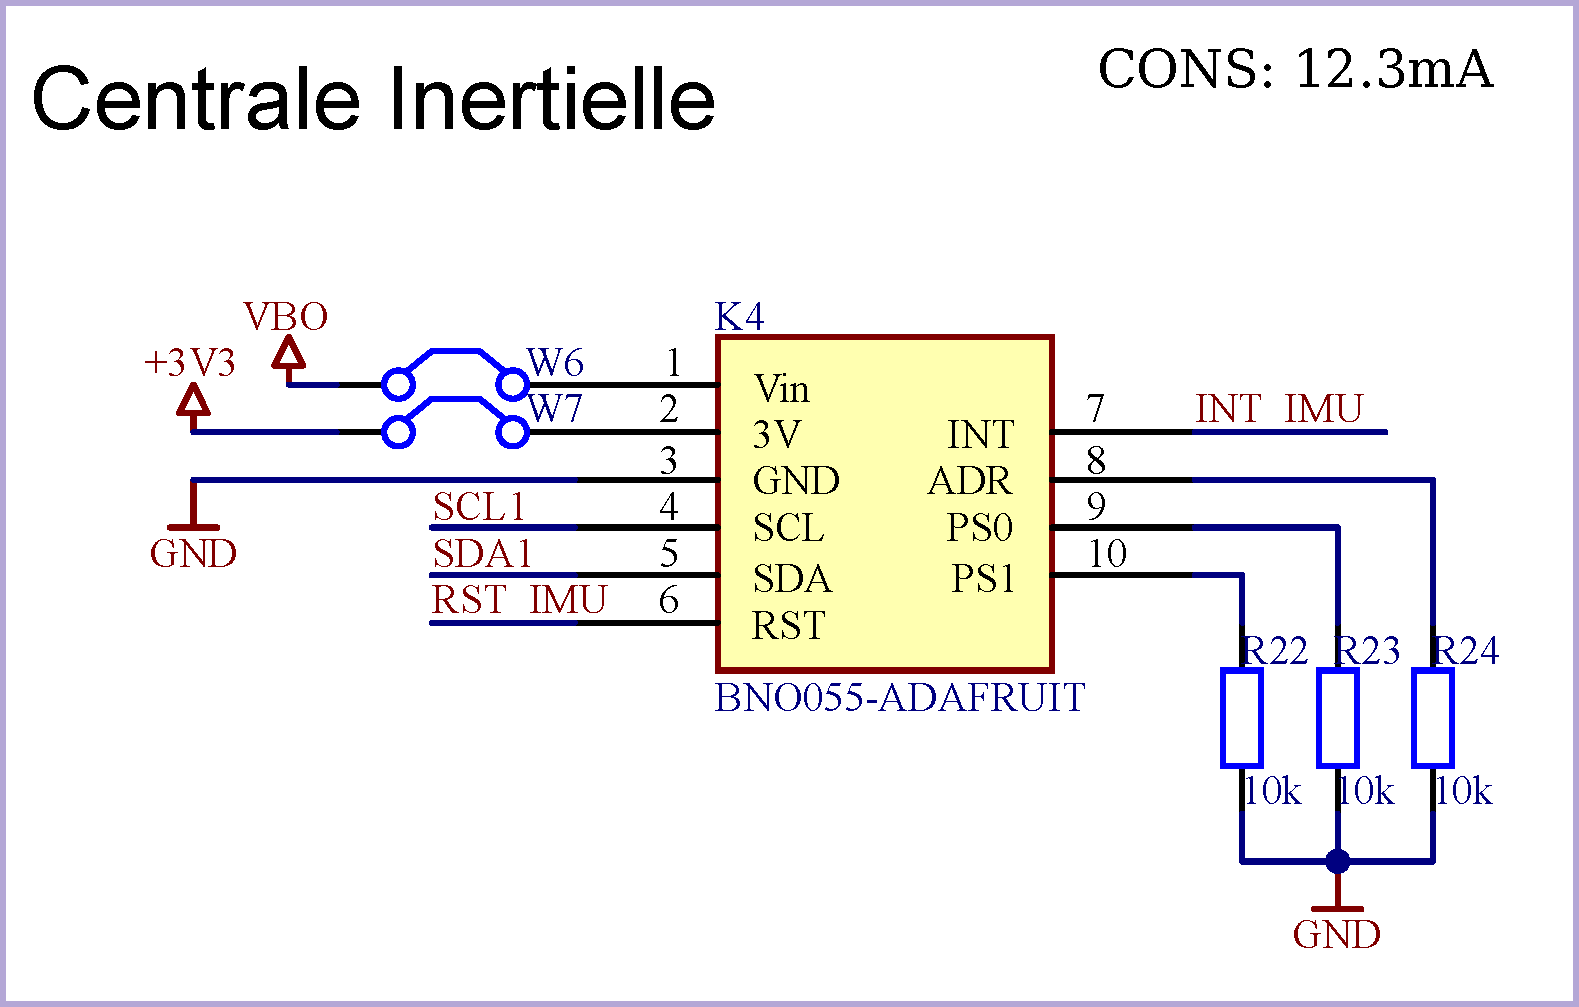
\includegraphics[width=0.5\linewidth]{../figures/etude/sch/IMU}
	\caption{Schéma centrale inertielle.}
	\source{Auteur}
	\label{fig:imu}
\end{figure}

La centrale inertielle, étant déjà montée sur une carte d'extension, ne nécessite pas de composants passifs additionnels. Trois résistances de PULL-DOWN sont présentes, respectivement sur \textbf{ADR}, \textbf{PS0} et \textbf{PS1}. Elles permettent de configurer l'adresse et l'interface de communication de l'\gls{imu}. De plus, un jumper\footnote{Connecteur permettant de faire ou de rompre une connexion.} est présent sur les alimentations. Ceci permet de choisir si la centrale inertielle est alimentée indépendamment du reste du système (pour pouvoir l'allumer séparément) ou avec la même alimentation que le reste du système.


\subsubsection{GNSS}
\begin{figure}[h]
	\centering
	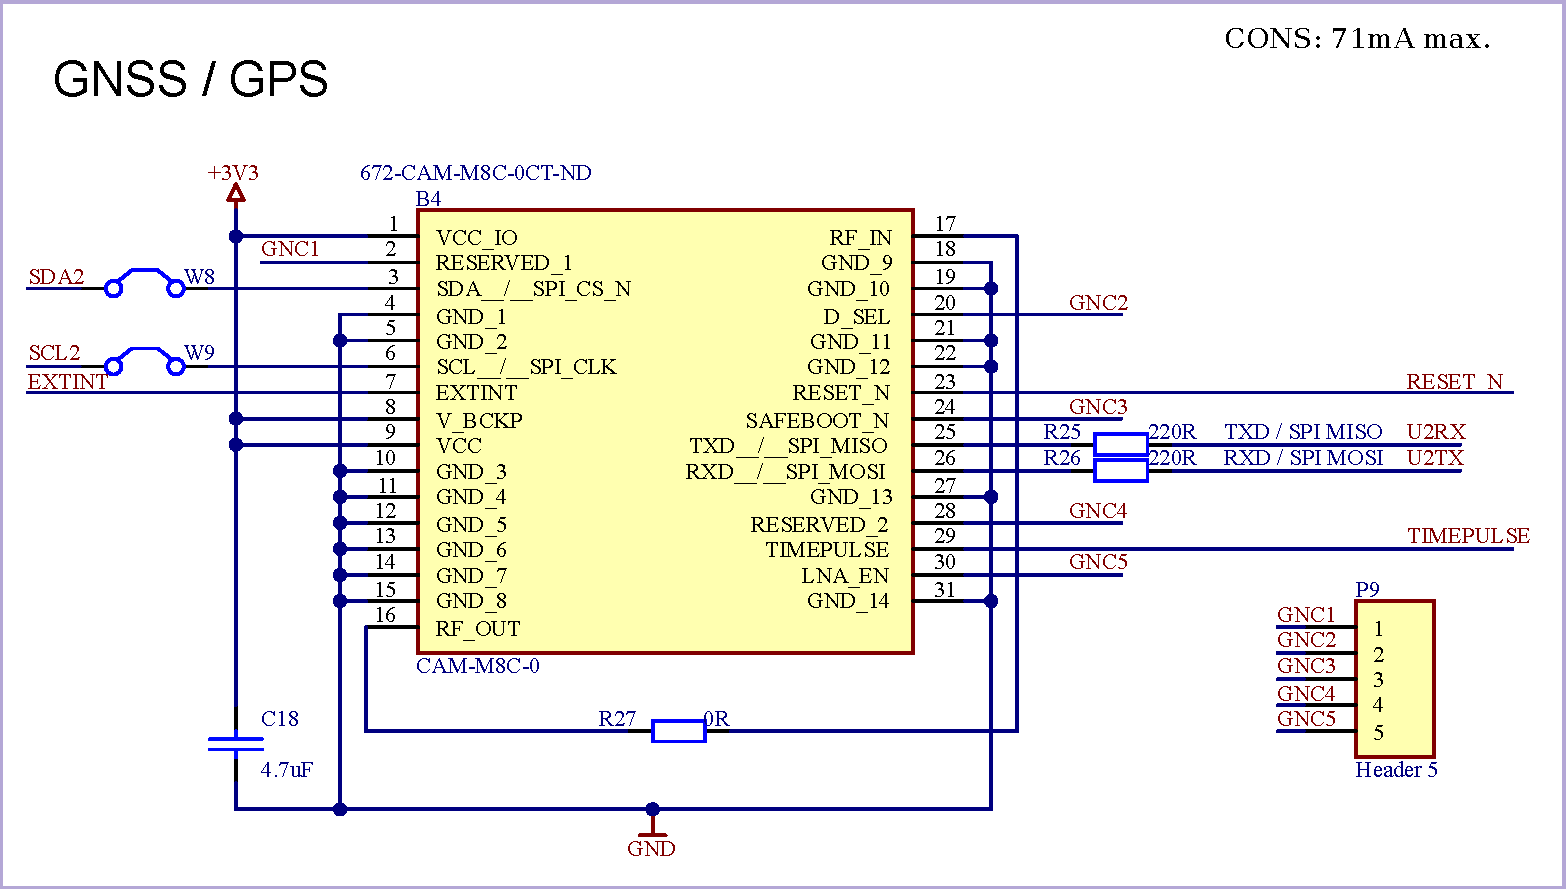
\includegraphics[width=.6\linewidth]{../figures/etude/sch/GNSS}
	\caption{Schéma du \gls{GNSS}.}
	\source{Auteur}
	\label{fig:gnss}
\end{figure}

Le \gls{GNSS} est connecté selon un schéma présenté dans son \href{https://www.u-blox.com/sites/default/files/CAM-M8-FW3_HIM_%28UBX-15030063%29.pdf}{Hardware Integration Manual}, à la section \textbf{2.2}. Ce schéma représente un design minimal pour recevoir des données via l'interface UART. Par rapport à la figure \ref{fig:gnss}, les différences sont les suivantes : l'interface I2C est également disponible, la PIN \textbf{RESET\_N} est connectée au \gls{mcu} et les PINS non-utilisées sont reliées à un connecteur afin de permettre leur utilisation éventuelle dans le cadre du prototype.

\subsubsection{USB - FTDI}

\begin{figure}[h]
	\centering
	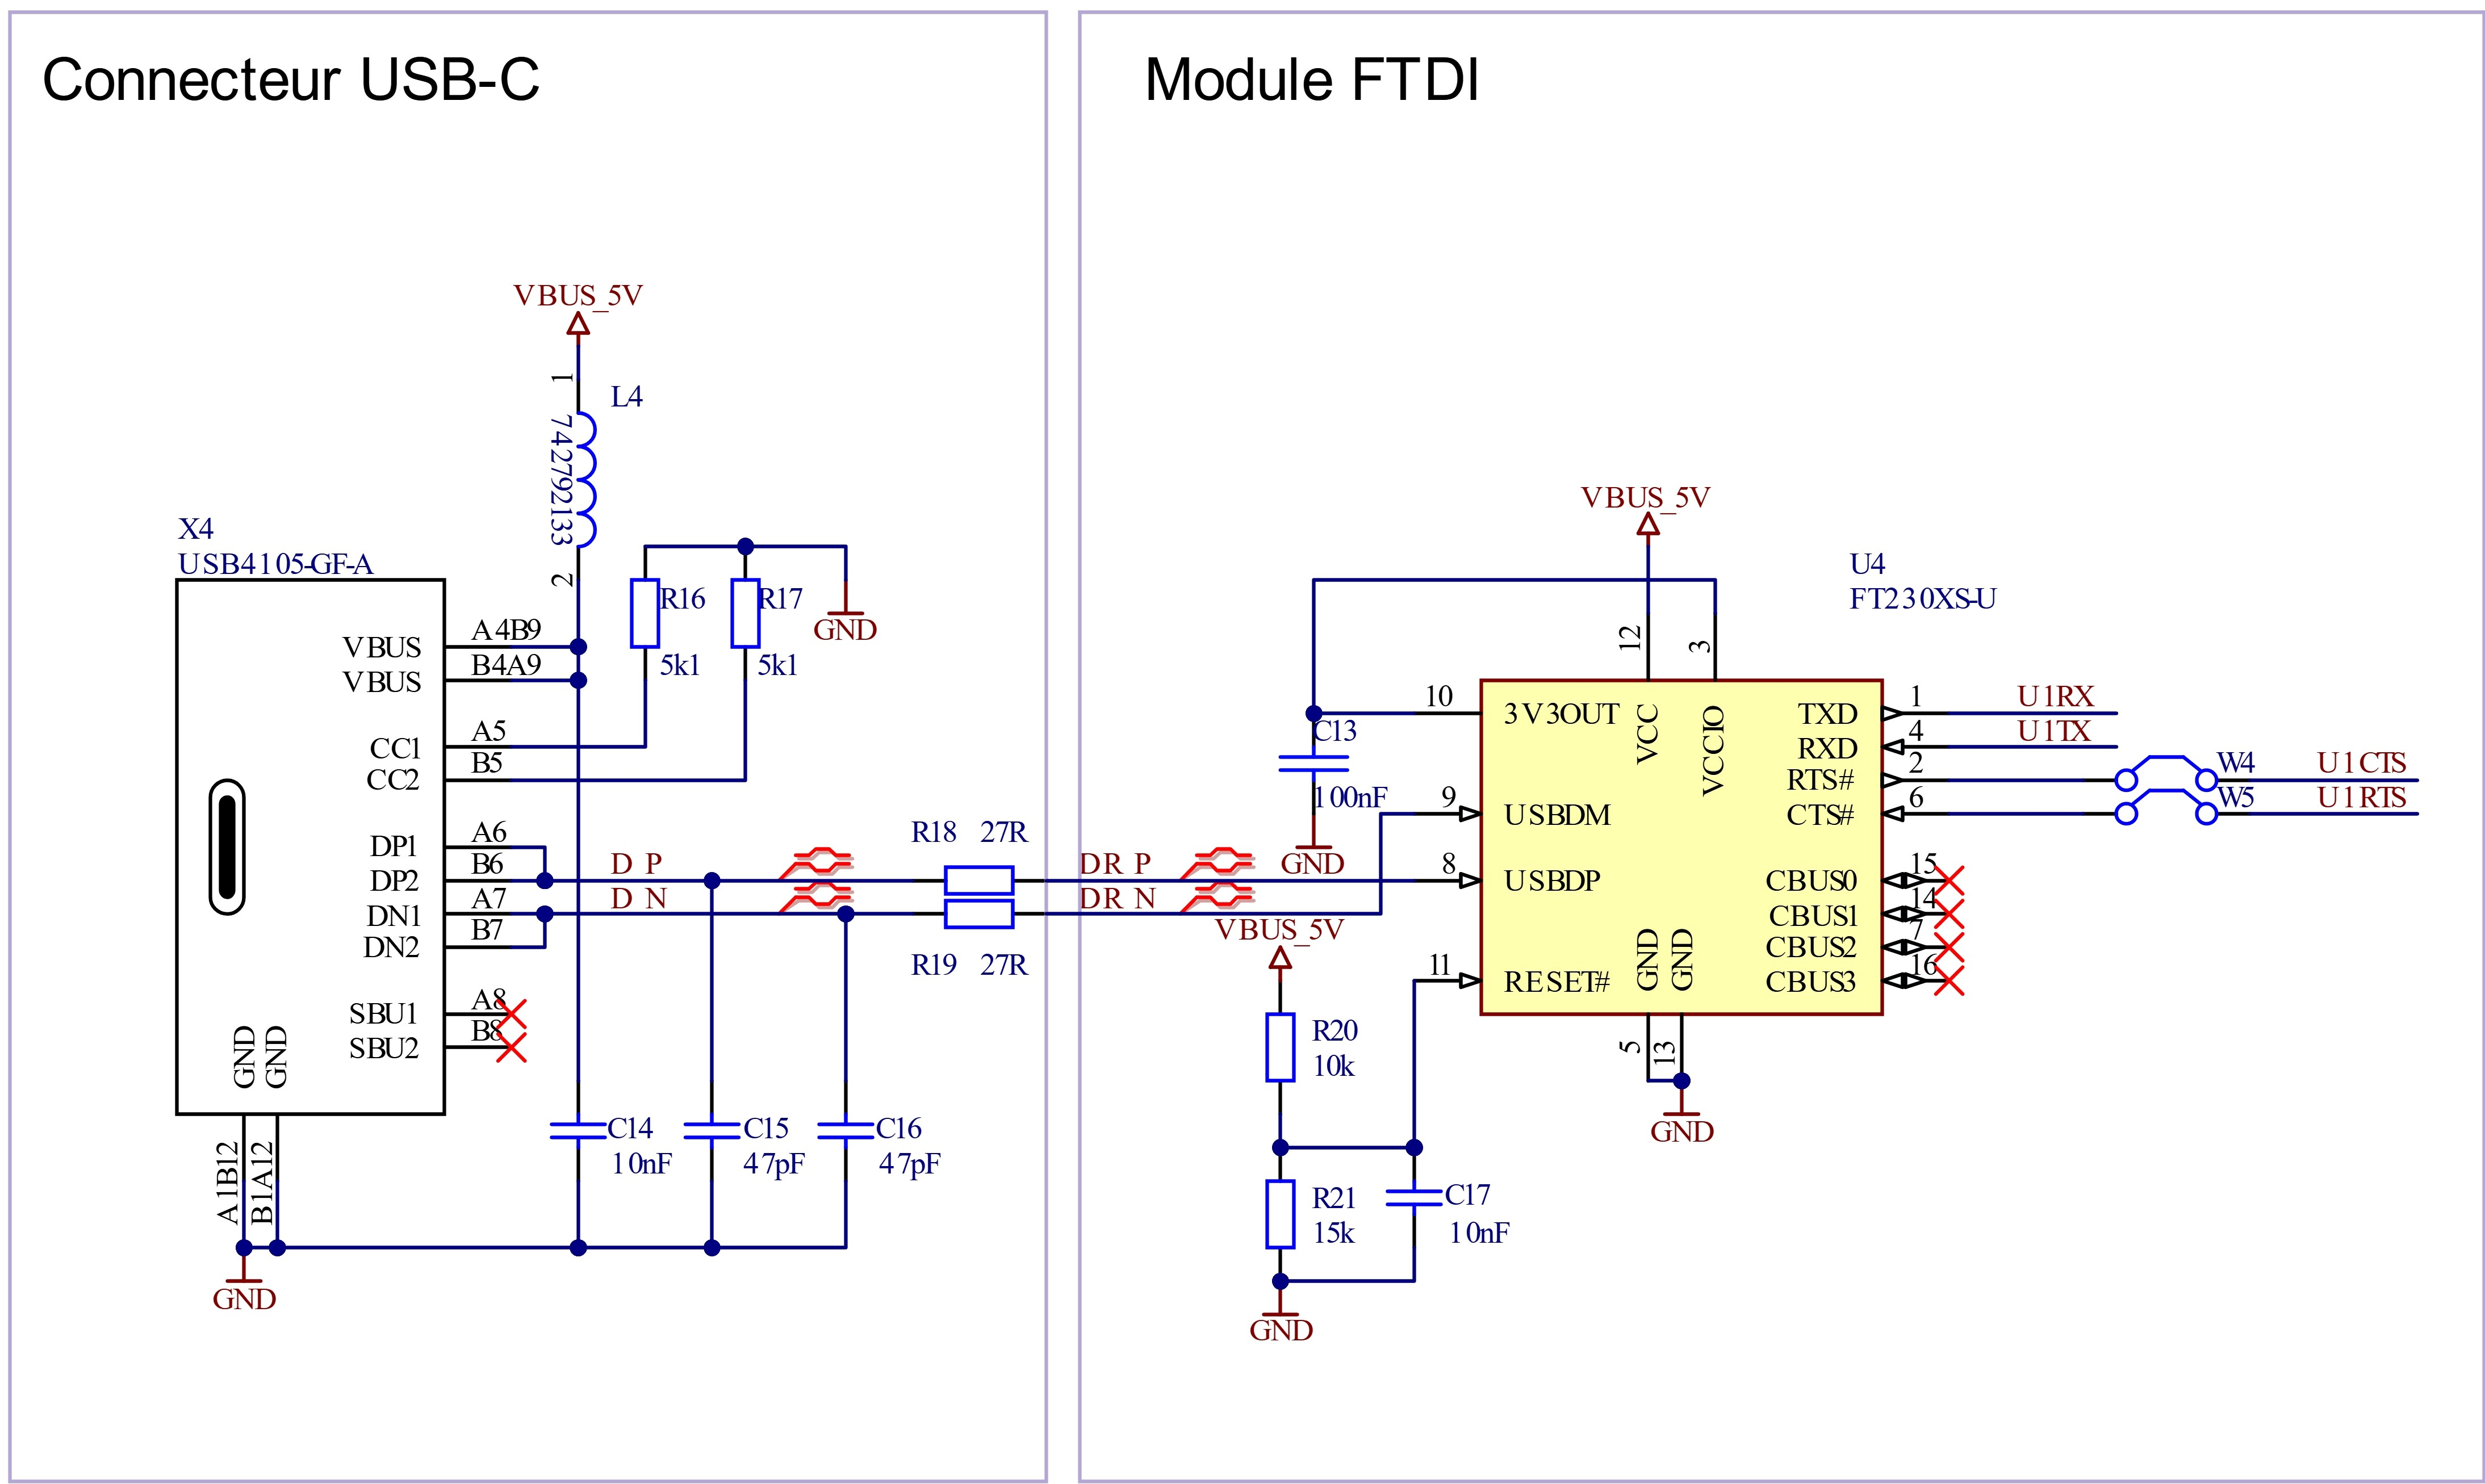
\includegraphics[width=.8\linewidth]{../figures/etude/sch/USB-FTDI}
	\caption{Schéma connecteur USB et FTDI.}
	\source{Auteur}
	\label{fig:usb-ftdi}
\end{figure}

Le schéma du connecteur USB-C est conçu pour présenter une résistance aux interférences. Son signal 5V est filtré par une \textit{ferrite bead}. Les pistes différentielles de l'USB sont ensuite reliées au module \gls{FTDI}, qui est interfacé en UART et est alimenté par l'USB.

\clearpage

\subsection{Alimentations} \label{ssec:Dev-Alim}
Dans cette section, nous allons décrire les fonctionnement et dimensionnements principaux du bloc alimentation comprenant les différents régulateurs et la batterie.

\subsubsection{Chargeur de batterie} \label{sssec:Chargeur-bat}

\begin{figure}[h]
	\centering
	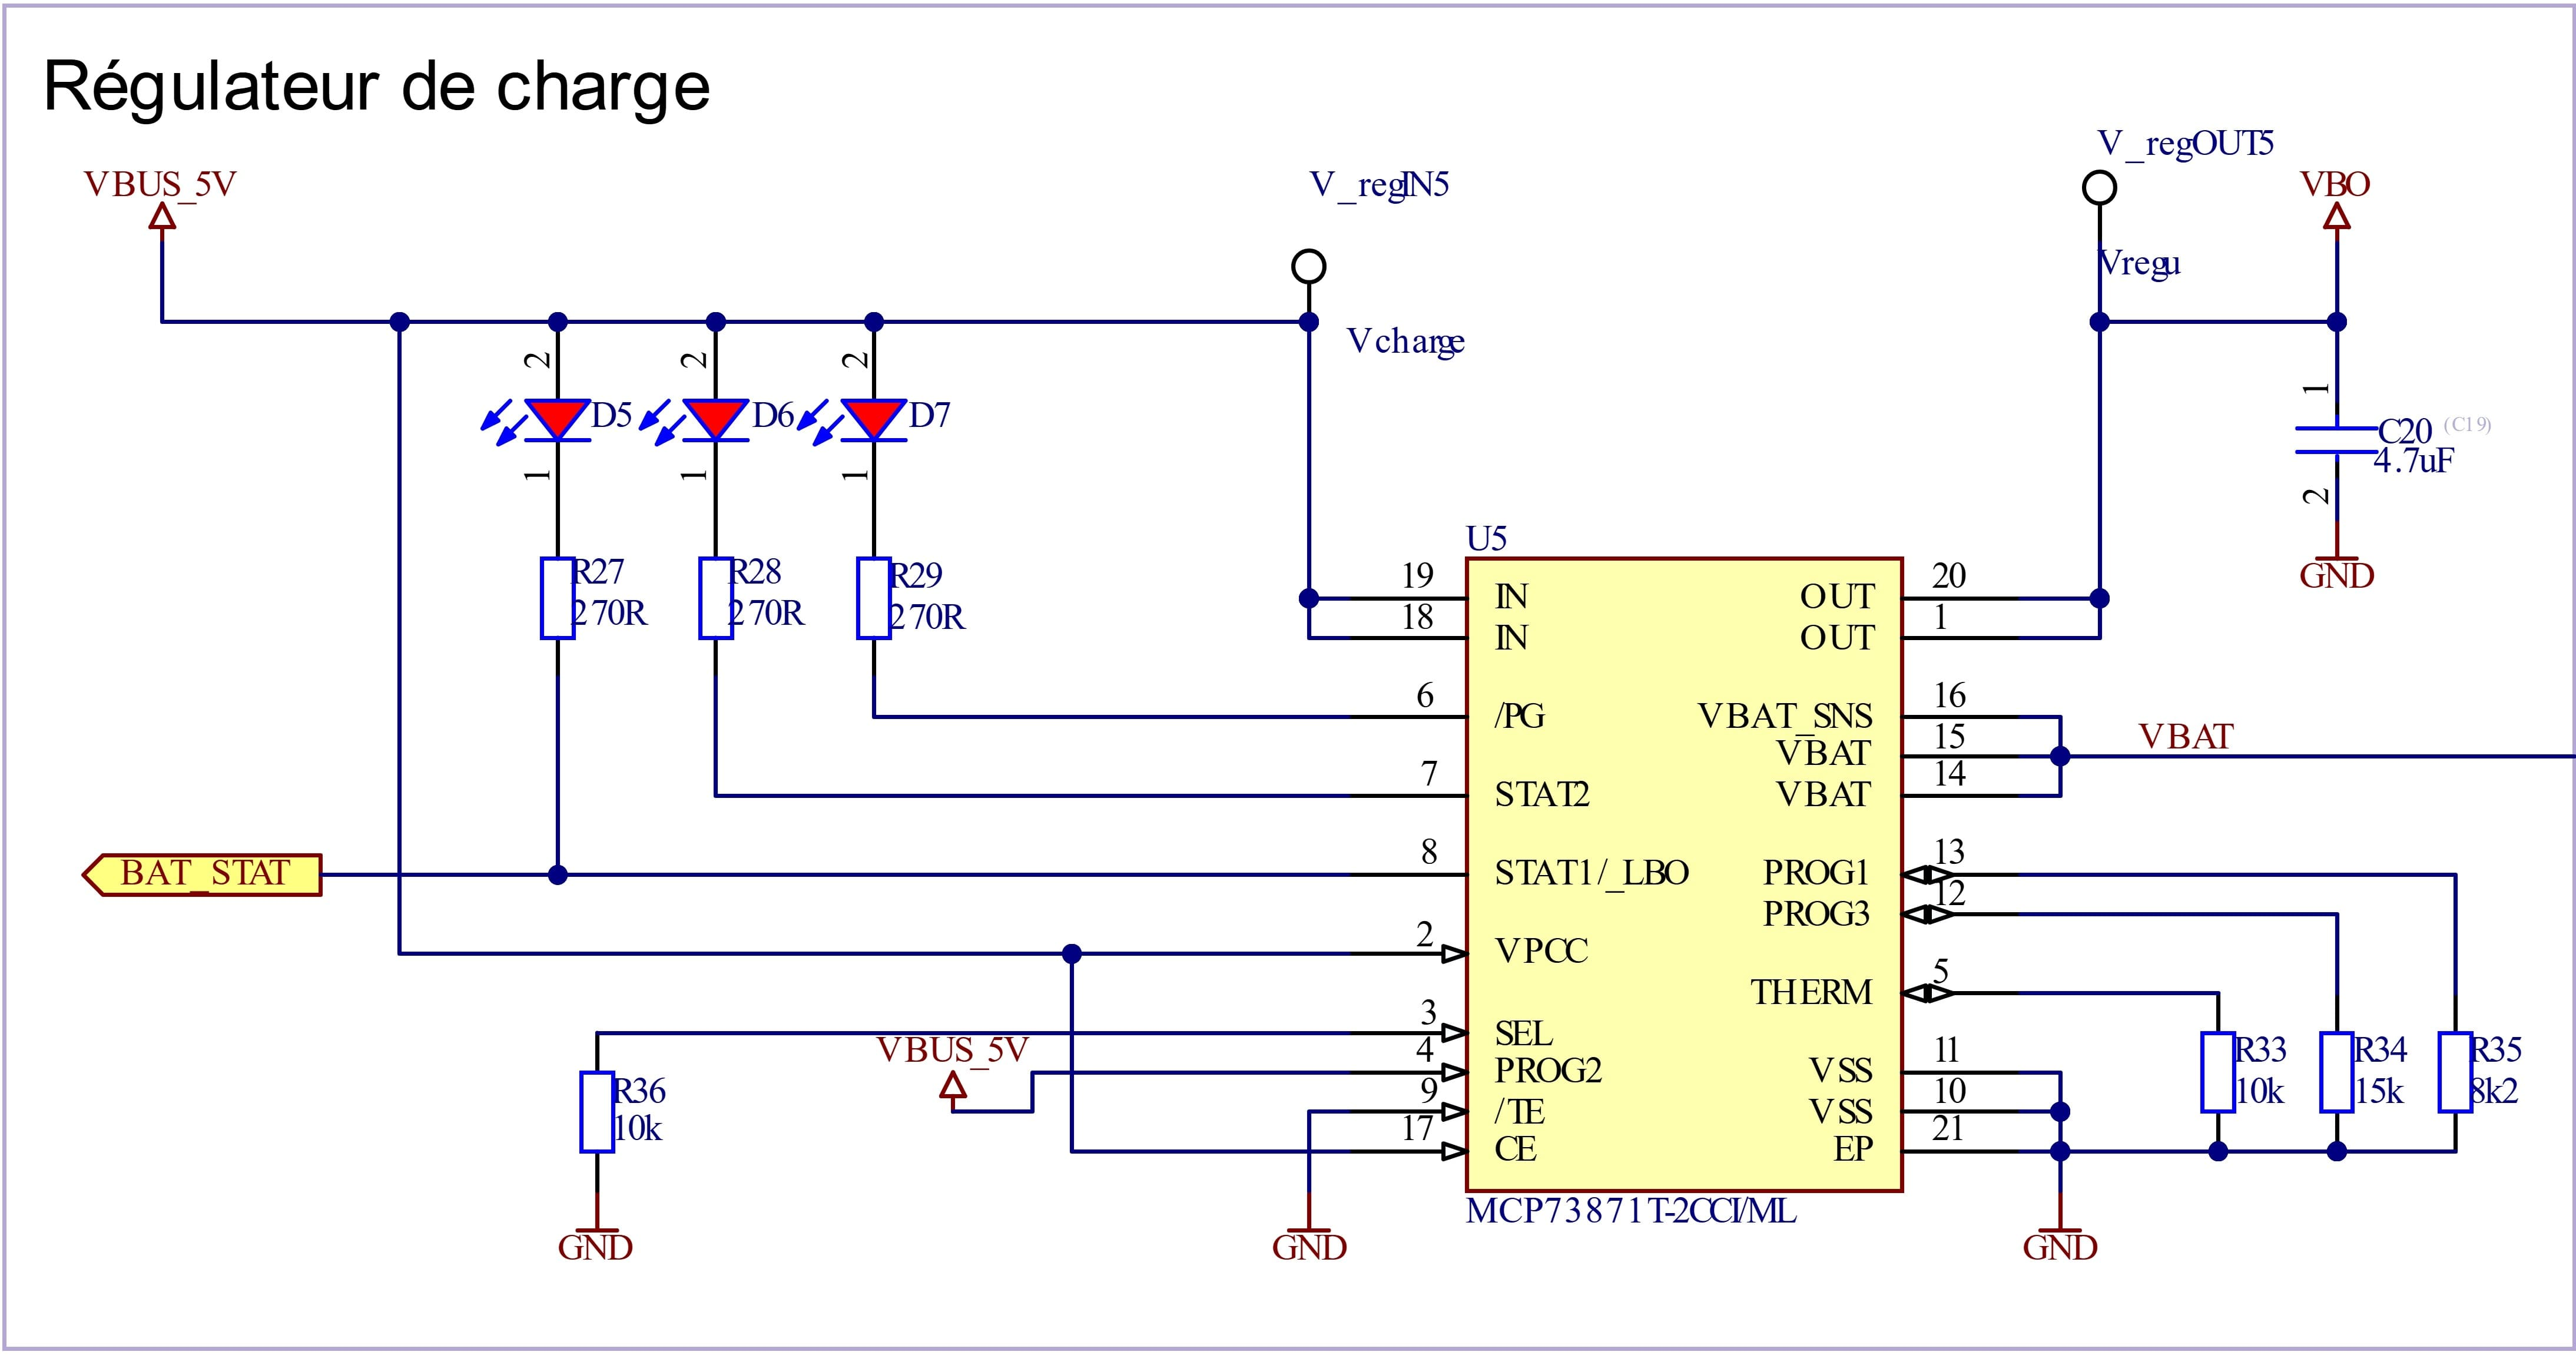
\includegraphics[width=.93\linewidth]{../figures/etude/sch/CHRG-BAT}
	\caption{Schéma chargeur de batterie.}
	\source{Auteur}
	\label{fig:chrg-bat}
\end{figure}

Le composant \textbf{MCP73871T-2CCI/ML} est configurable pour délivrer un courant de charge programmable à la batterie. Ce courant se sépare en deux phases : la charge normale et la charge de terminaison. Cette dernière est activée lorsque la batterie approche de sa capacité maximale. Pour déterminer ces courants, il convient de se baser sur la capacité de la batterie et de certains ratios standards associés.

Où :

$C = 1600 mAh$ est la capacité de la batterie.

$k_{term} = 0.05$ est le ratio de fin de charge.

$k_{chg} = 0.15$ est le ratio de charge.

Le courant de terminais peut être calculé ainsi :
\begin{equation*}
	I_{term} = C * k_{term} = 1600 * 0.05 = 80 \; mA
\end{equation*}
Par conséquent, d'après la \gls{datasheet} (\href{https://ww1.microchip.com/downloads/en/DeviceDoc/MCP73871-Data-Sheet-20002090E.pdf}{Equation 4-2}) la résistance de programmation de fin de charge vaudrait :
\begin{equation*}
	R_{prog3} = \frac{1000V}{I_{term}} = \frac{1000}{65*10^{-3}} = 12.5 \; k\Omega \Rightarrow 12 \; k\Omega
\end{equation*}
Nous pouvons de la même facon cacluler la résistance de charge \textbf{Rprog1} :
\begin{equation*}
	R_{prog1} = \frac{1000V}{C*k_{chg}} = \frac{1000}{1600*10^{-3}*0.15} = 4.166 \; k\Omega \Rightarrow 3.9 \; k\Omega
\end{equation*}

\clearpage

\subsubsection{Système d'enclenchement} \label{sssec:On-OFF}


\begin{figure}[h]
	\centering
	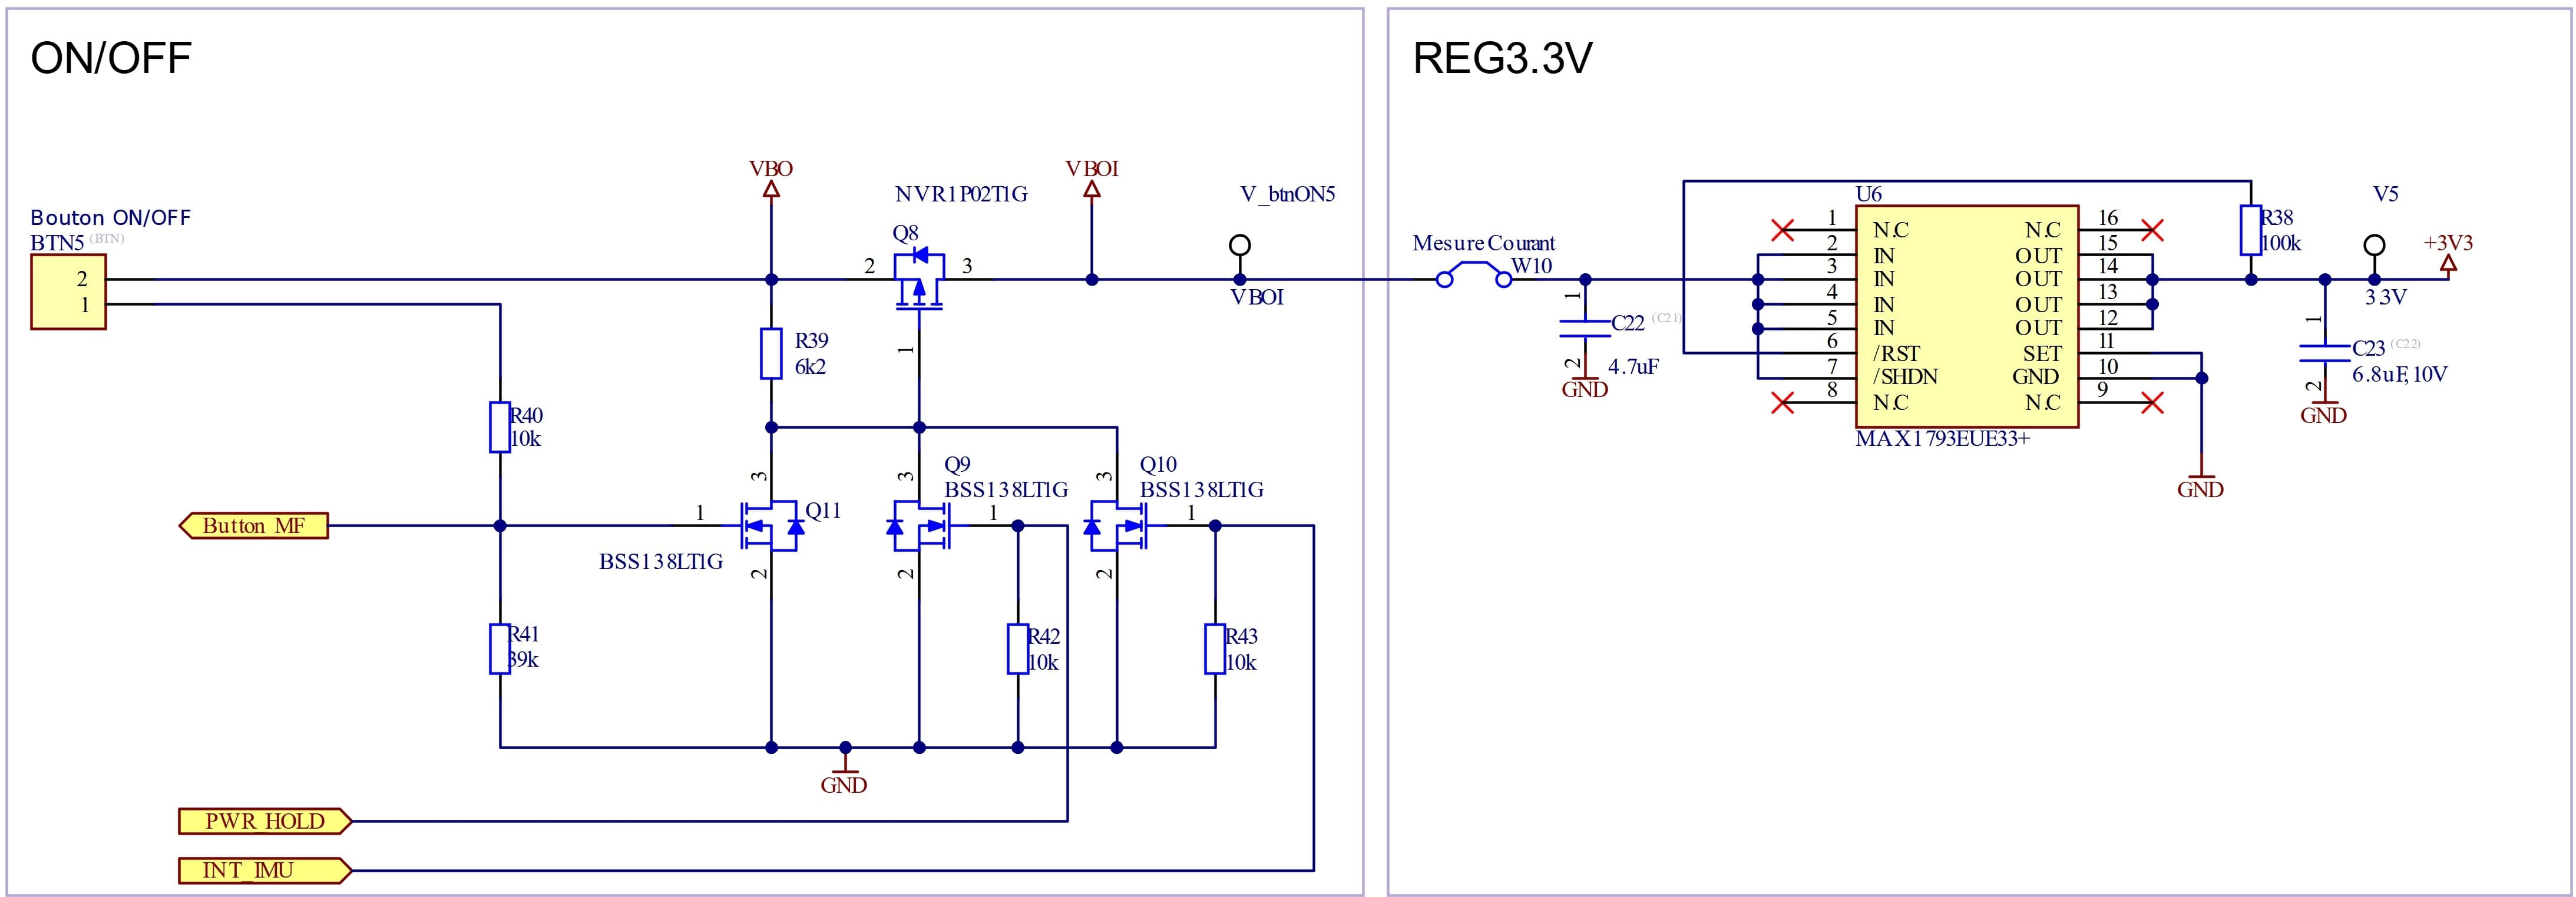
\includegraphics[width=1\linewidth]{../figures/etude/sch/ON-OFF}
	\caption{Schéma allumage du système.}
	\source{Auteur}
	\label{fig:on-off}
\end{figure}

Sur la figure \ref{fig:on-off}, nous observons les différentes manières de connecter la tension régulée de la batterie au régulateur linéaire \textbf{3.3V}. Quand cette connexion n'est pas réalisée, le système n'est pas alimenté, à l'exception de l'\gls{imu} qui peut être alimenté de manière autonome. Pour mettre en marche le système, trois options sont possibles : \vspace{2mm}

\begin{itemize}
	\item[\faChevronRight] Le microcontrôleur peut maintenir le système alimenté avec \textbf{PWR\_HOLD}. 
	\item[\faChevronRight] L'\gls{imu} peut 'allumer le système avec son interruption \textbf{INT\_IMU}. 
	\item[\faChevronRight] Un bouton peut être préssé pour enclencher la carte \textbf{Button\_MF}. 
\end{itemize}

\subsection{Conclusion et perspectives de l'étude} \label{ssec:Conclusion-etude}

Tout au long de cette étude, nous avons pu décomposer et analyser le processus de développement du schéma électronique. La démarche a priorisé la modularité, avec une division du système en trois blocs : \hyperref[ssec:Dev-MCU]{\textbf{Microcontrôleur \ref{ssec:Dev-MCU}}}, \hyperref[ssec:Dev-Devices]{\textbf{Périphériques \ref{ssec:Dev-Devices}}} et \hyperref[ssec:Dev-Alim]{\textbf{Alimentations \ref{ssec:Dev-Alim}}}. Cette approche a permis une meilleure lisibilité et une facilité d'adaptation quant au prototypage. Les différentes interactions et connexions entre les composants ont été détaillées.

Par la suite, le circuit imprimé sera développé, les composant placés et routés le tout dans un design petit et compact. La modularité du projet, permettra des tests empiriques sur les différents blocs du système, lors de la mise en service.


